%%%%%%%%%%%%%%%%%%%%%%%%%%%%%%%%%%%%%%%%%%%%%%%%%%%%%%%%%%%%%%%%%%%%%%%%%%%%%%%%
\chapter{KPI Degradation Analyzer}
\label{chap:kpi_degradation}

The KPI Degradation Analyzer is the first and most comprehensive analytical module of the RANPilotAI platform. It is designed to automatically detect, classify, and localise Key Performance Indicator degradations across LTE and 5G NR Radio Access Networks using a statistically-aware, three-layer analytical pipeline. The module processes tabular KPI counter exports, applies data quality validation, computes degradation magnitudes against historical baselines, and performs RF-aware root cause analysis to produce actionable engineering output for each degraded cell.

The module supports 13 KPI categories spanning all five standard pillars of RAN performance: accessibility, retainability, mobility, integrity, and availability. The root cause analysis engine applies over 140 correlated detection rules encoding domain-specific RF engineering knowledge, producing structured output that includes degradation severity classification, statistical confidence scoring, root cause pattern identification, and recommended next investigation steps.

%%%%%%%%%%%%%%%%%%%%%%%%%%%%%%%%%%%%%%%%%%%%%%%%%%%%%%%%%%%%%%%%%%%%%%%%%%%%%%%%
\section{Introduction}

Modern LTE and 5G NR base stations generate performance management counter data at regular intervals, typically every 15 minutes or hourly. For a network of even moderate size, this results in datasets containing tens of thousands of rows and hundreds of columns, with each cell contributing observations across dozens of KPI categories \cite{holma2011}. Identifying which cells are degraded, quantifying the severity of the degradation, and determining the probable root cause requires correlating the degraded KPI against a set of related diagnostic counters using engineering expertise that is difficult to systematise and impossible to apply consistently at network scale through manual methods.

The KPI Degradation Analyzer addresses this challenge by implementing a fully automated three-layer analytical pipeline that processes raw KPI counter exports and produces structured degradation reports without requiring manual cell-by-cell inspection. The module is implemented as a Streamlit-based interactive application that enables engineers to configure analysis parameters, upload data, initiate analysis, and explore results through an interactive tabular and graphical interface.

Figure~\ref{fig:analyzer_interface} presents the initial state of the KPI Degradation Analyzer interface before data is loaded. The interface displays the tool header with its four capability tags, the sidebar data source upload panel, and the four analytical capability cards describing the available analysis functions.

\begin{figure}[H]
    \centering
    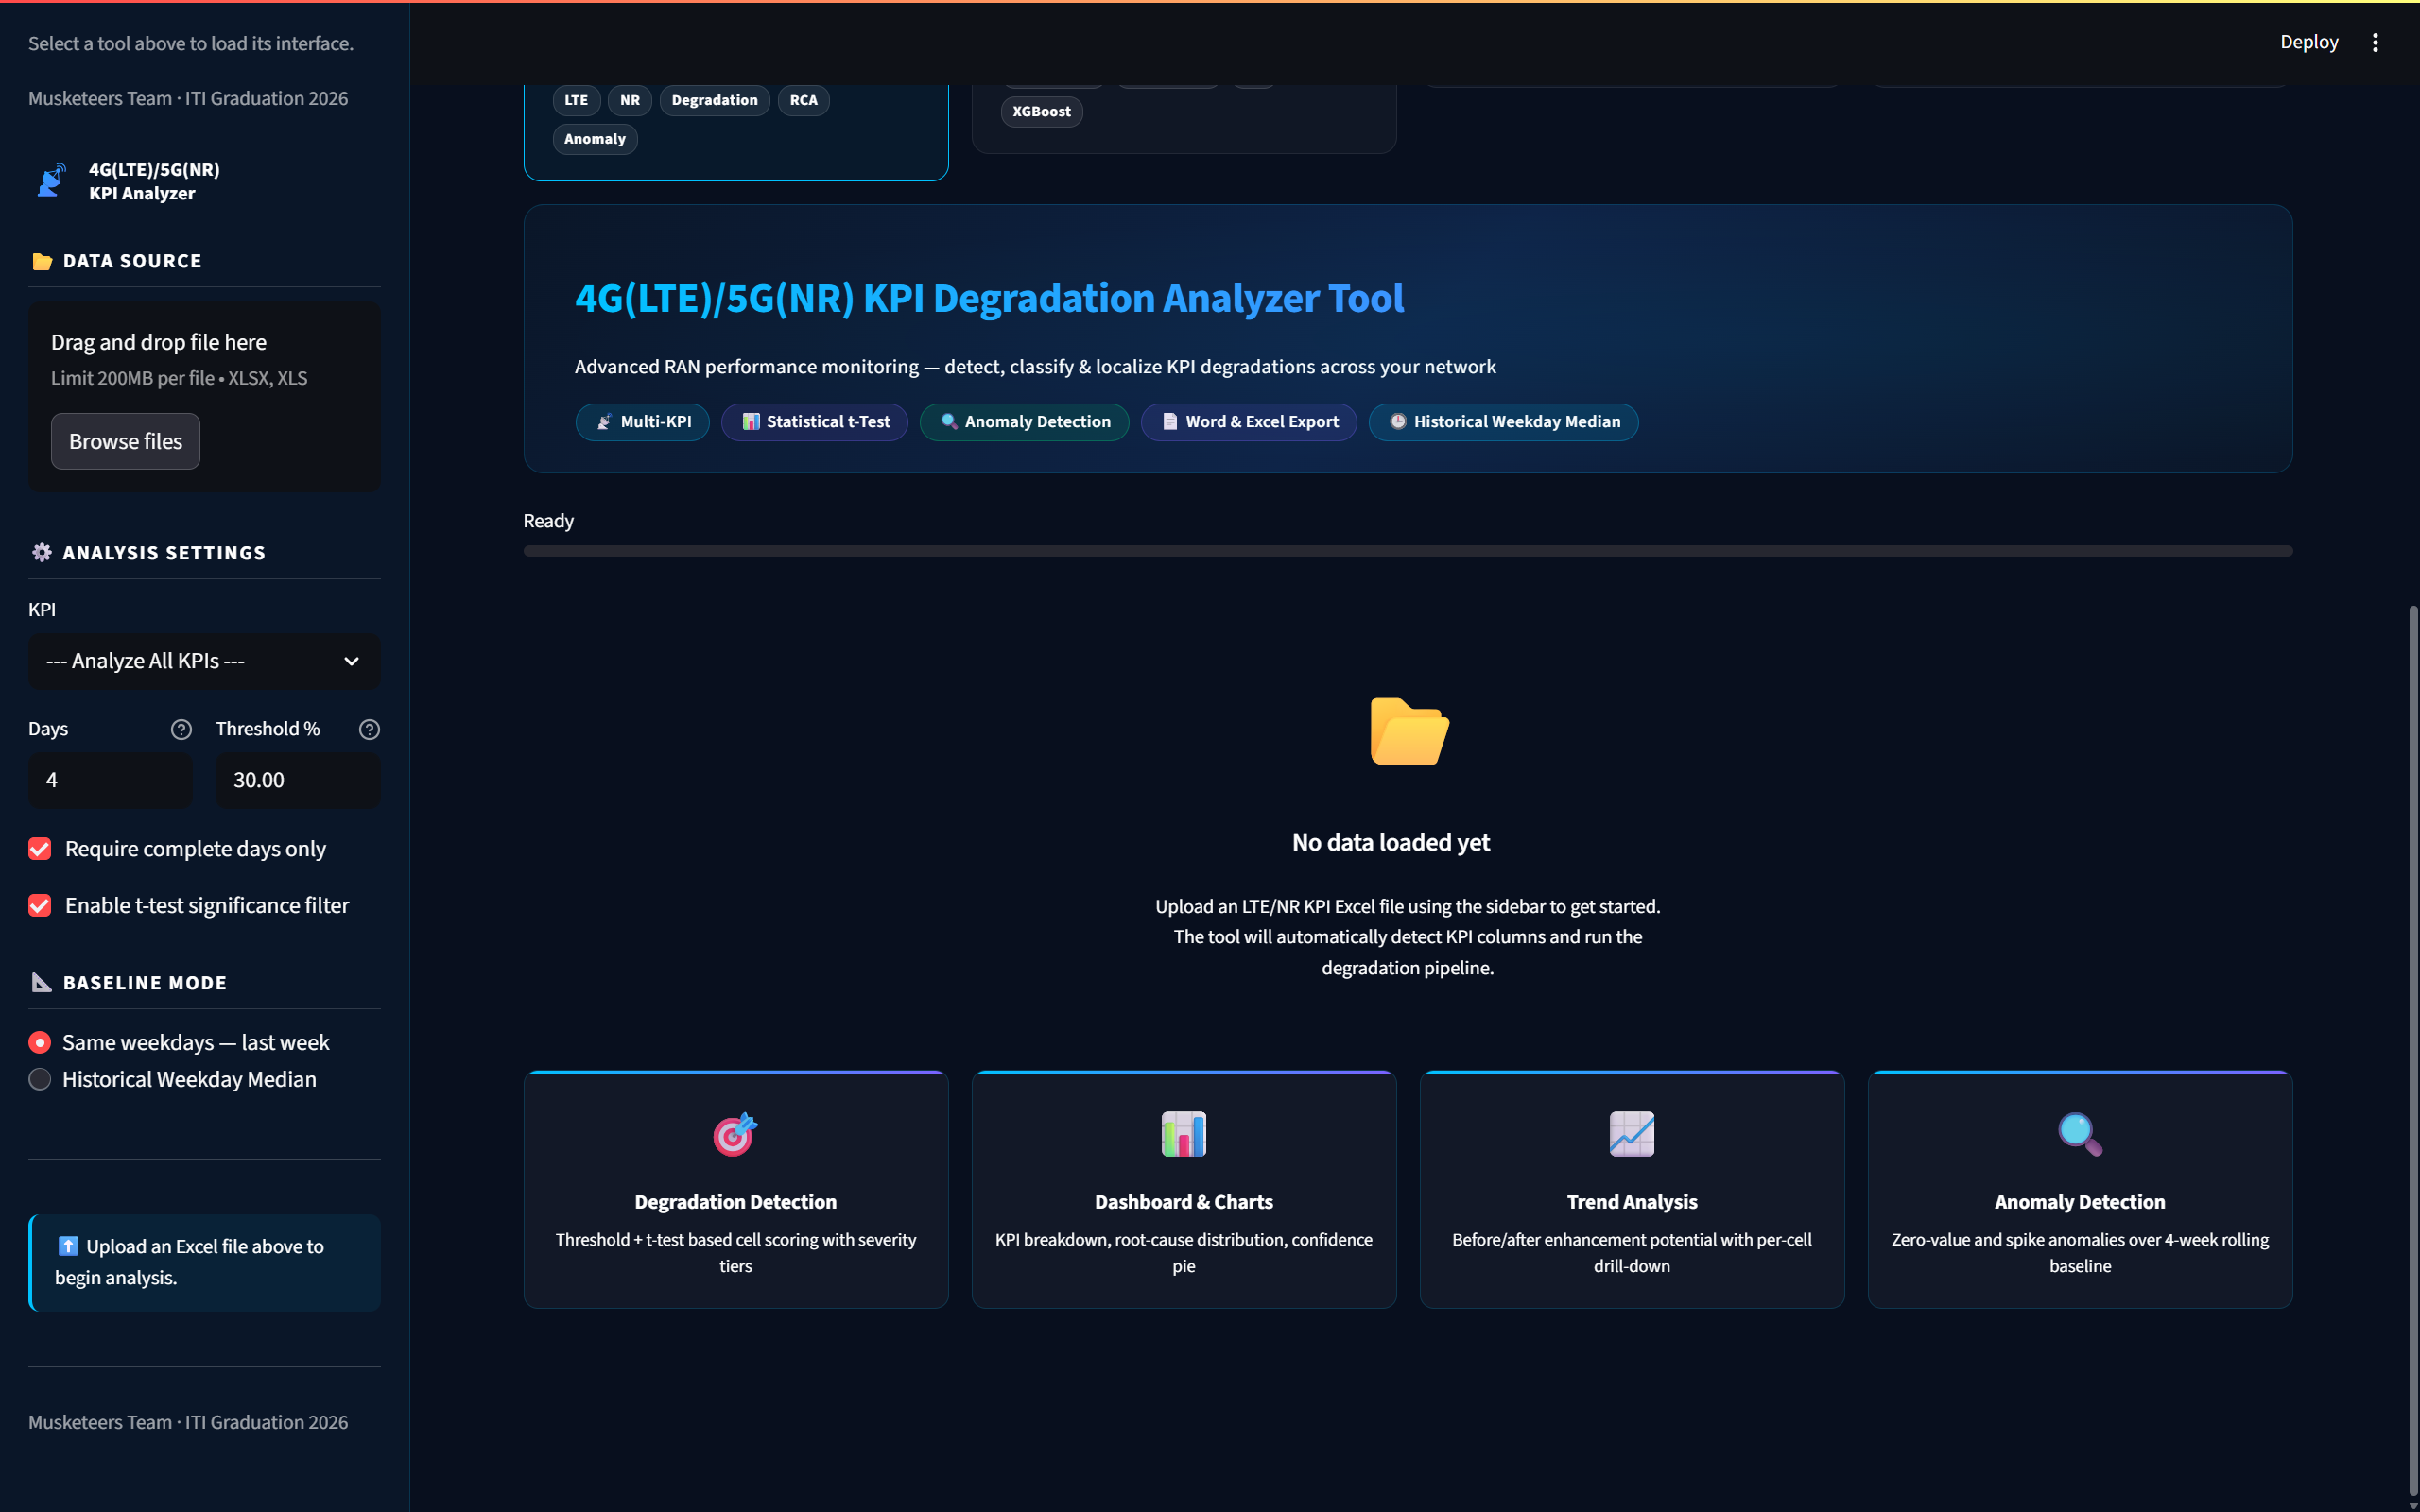
\includegraphics[width=\textwidth]{figures/chapter04/analyzer_interface.png}
    \caption{Initial interface of the KPI Degradation Analyzer module showing the tool header, sidebar data source and analysis settings panel, and the four capability cards: Degradation Detection, Dashboard \& Charts, Trend Analysis, and Anomaly Detection.}
    \label{fig:analyzer_interface}
\end{figure}

%%%%%%%%%%%%%%%%%%%%%%%%%%%%%%%%%%%%%%%%%%%%%%%%%%%%%%%%%%%%%%%%%%%%%%%%%%%%%%%%
\section{Motivation}

The operational motivation for developing an automated KPI degradation detection module arises directly from the limitations of existing manual analysis workflows in commercial network operations centres.

In a typical manual workflow, an RF engineer downloads a weekly KPI report from the network management system, opens it in a spreadsheet application, applies filters and conditional formatting to identify cells exceeding predefined thresholds, and then manually examines the counter values for each flagged cell to determine the root cause. This process is time-consuming, requires sustained concentration, and relies entirely on the individual engineer's domain knowledge and experience to produce consistent root cause classifications.

Furthermore, threshold-based alerting — the primary automated mechanism available in most commercial network management systems — suffers from two fundamental limitations. First, a fixed threshold applied uniformly across all cells ignores the natural variability and baseline performance level of each individual cell. A threshold of 95\% for RRC Setup Success Rate may correctly flag a degraded urban macro cell while missing a structural degradation in a rural small cell with a historically lower baseline. Second, threshold crossing alone provides no information about the probable root cause of the degradation, leaving the full diagnostic burden on the engineer.

The KPI Degradation Analyzer replaces this manual workflow with an automated pipeline that applies cell-specific historical baselines, computes statistically-aware degradation magnitudes, and correlates degraded KPIs against RF-aware root cause patterns to produce a complete, structured analysis report in seconds.

%%%%%%%%%%%%%%%%%%%%%%%%%%%%%%%%%%%%%%%%%%%%%%%%%%%%%%%%%%%%%%%%%%%%%%%%%%%%%%%%
\section{Problem Statement}

The technical challenge addressed by the KPI Degradation Analyzer encompasses three distinct sub-problems.

\textbf{Data quality}: Real-world KPI exports from vendor network management systems contain numerous data quality artefacts that must be detected and handled before statistical analysis can be applied. These include sentinel values — large integer constants such as 4{,}294{,}967{,}295 and 4{,}294{,}967{,}294 used by Huawei systems to indicate counter unavailability — negative values in counters that should be non-negative, values exceeding theoretical bounds for percentage KPIs, cells with incomplete observation windows, and mixed units within a single column due to vendor export configurations. Failure to detect and remove these artefacts before analysis produces incorrect degradation magnitudes and false root cause assignments.

\textbf{Degradation quantification}: Different KPI types require different mathematical treatment when computing degradation magnitude. Counter KPIs such as traffic volume and throughput are best expressed as relative percentage changes from baseline: $(B - R) / B \times 100$, where $B$ is the baseline mean and $R$ is the recent mean. Ratio KPIs such as RRC Setup Success Rate, E-RAB Drop Rate, and Handover Success Rate are better expressed as signed percentage-point differences: $R - B$, which avoids divide-by-zero conditions when the baseline approaches zero and provides a physically more meaningful magnitude for binary success rate metrics.

\textbf{Root cause attribution}: Determining the probable root cause of a detected KPI degradation requires correlating the degraded KPI against a specific set of related diagnostic counters. The appropriate set of diagnostic counters, the directionality of the correlation, and the severity weighting assigned to each correlated counter depend on the KPI category, the direction of degradation, the RF technology, and the deployment context. Encoding this domain knowledge as a systematic, extensible rule set that produces consistent results across all cells and KPI categories is the central engineering challenge of the root cause analysis engine.

%%%%%%%%%%%%%%%%%%%%%%%%%%%%%%%%%%%%%%%%%%%%%%%%%%%%%%%%%%%%%%%%%%%%%%%%%%%%%%%%
\section{Background}

\subsection{KPI Categories and Performance Pillars}

The KPI Degradation Analyzer monitors 13 KPI categories aligned with the five standard performance pillars used in LTE and 5G NR network assessment. Table~\ref{tab:kpi_categories} summarises the monitored KPI categories, their associated performance pillars, and the direction of degradation for each.

\begin{table}[H]
    \centering
    \caption{KPI categories monitored by the KPI Degradation Analyzer.}
    \label{tab:kpi_categories}
    \begin{tabular}{|c|l|l|l|}
        \hline
        \textbf{\#} & \textbf{KPI Category} & \textbf{Pillar} & \textbf{Bad Direction} \\
        \hline
        1  & DL Traffic Volume    & Traffic         & Low  \\
        2  & UL Traffic Volume    & Traffic         & Low  \\
        3  & DL Throughput        & Integrity       & Low  \\
        4  & UL Throughput        & Integrity       & Low  \\
        5  & RRC Setup SR         & Accessibility   & Low  \\
        6  & E-RAB Setup SR       & Accessibility   & Low  \\
        7  & E-RAB Drop Rate      & Retainability   & High \\
        8  & HO Success Rate      & Mobility        & Low  \\
        9  & Cell Availability    & Availability    & Low  \\
        10 & RACH Success Rate    & Accessibility   & Low  \\
        11 & CSFB KPIs            & Accessibility   & Low  \\
        12 & VoLTE KPIs           & Integrity       & Varies \\
        13 & RRC Re-establishment & Retainability   & High \\
        \hline
    \end{tabular}
\end{table}

\subsection{Welch's t-test for Degradation Confidence}

The module employs Welch's two-sample t-test as an advisory statistical confidence measure when comparing recent KPI observations against the historical baseline \cite{montgomery2018}. Welch's test is preferred over the standard Student's t-test because it does not assume equal variance between the recent observation window and the baseline window, which is a commonly violated assumption in KPI degradation scenarios where the degradation period is characterised by increased variance.

The test statistic is computed as:

\begin{equation}
    t = \frac{\bar{x}_{\text{recent}} - \bar{x}_{\text{baseline}}}{\sqrt{\dfrac{s_{\text{recent}}^2}{n_{\text{recent}}} + \dfrac{s_{\text{baseline}}^2}{n_{\text{baseline}}}}}
\end{equation}

The resulting p-value is used to assign a statistical confidence label — High, Medium, or Low — to each detected degradation. Critically, the p-value is treated as advisory evidence rather than as a hard gate: cells with operationally significant degradation magnitudes are retained in the output even when the statistical confidence is Low due to insufficient sample count in the observation window.

\subsection{RF-Aware Root Cause Scoring}

The root cause analysis engine assigns a composite score to each candidate root cause for a degraded cell using four additive components:

\begin{equation}
    \text{Score} = w_{\text{severity}} + w_{\text{RF\_priority}} + w_{\text{threshold}} + \min(w_{\text{magnitude}}, w_{\text{cap}})
\end{equation}

where $w_{\text{severity}}$ is the base severity weight assigned to the diagnostic counter type, $w_{\text{RF\_priority}}$ is a bonus applied to RF-layer counters reflecting their higher diagnostic priority, $w_{\text{threshold}}$ is a score increment applied when the counter value exceeds a predefined RF engineering threshold, $w_{\text{magnitude}}$ is a score component proportional to the absolute deviation of the counter from its expected value, and $w_{\text{cap}}$ is an upper bound on the magnitude component to prevent a single extremely deviant counter from dominating the composite score.

The eight operational RCA patterns produced by the engine are: Outage, Congestion, Radio Quality, Coverage, Interference, Mobility, Demand, and Unknown. Each pattern has a KPI-specific triage order that prioritises checking higher-confidence root cause hypotheses before less likely ones.

%%%%%%%%%%%%%%%%%%%%%%%%%%%%%%%%%%%%%%%%%%%%%%%%%%%%%%%%%%%%%%%%%%%%%%%%%%%%%%%%
\section{Analysis Configuration}

Before initiating analysis, the engineer configures the analysis parameters through the sidebar panel. Figure~\ref{fig:analysis_configuration} illustrates the analysis configuration state after a KPI data file has been uploaded and the analysis settings have been configured.

\begin{figure}[H]
    \centering
    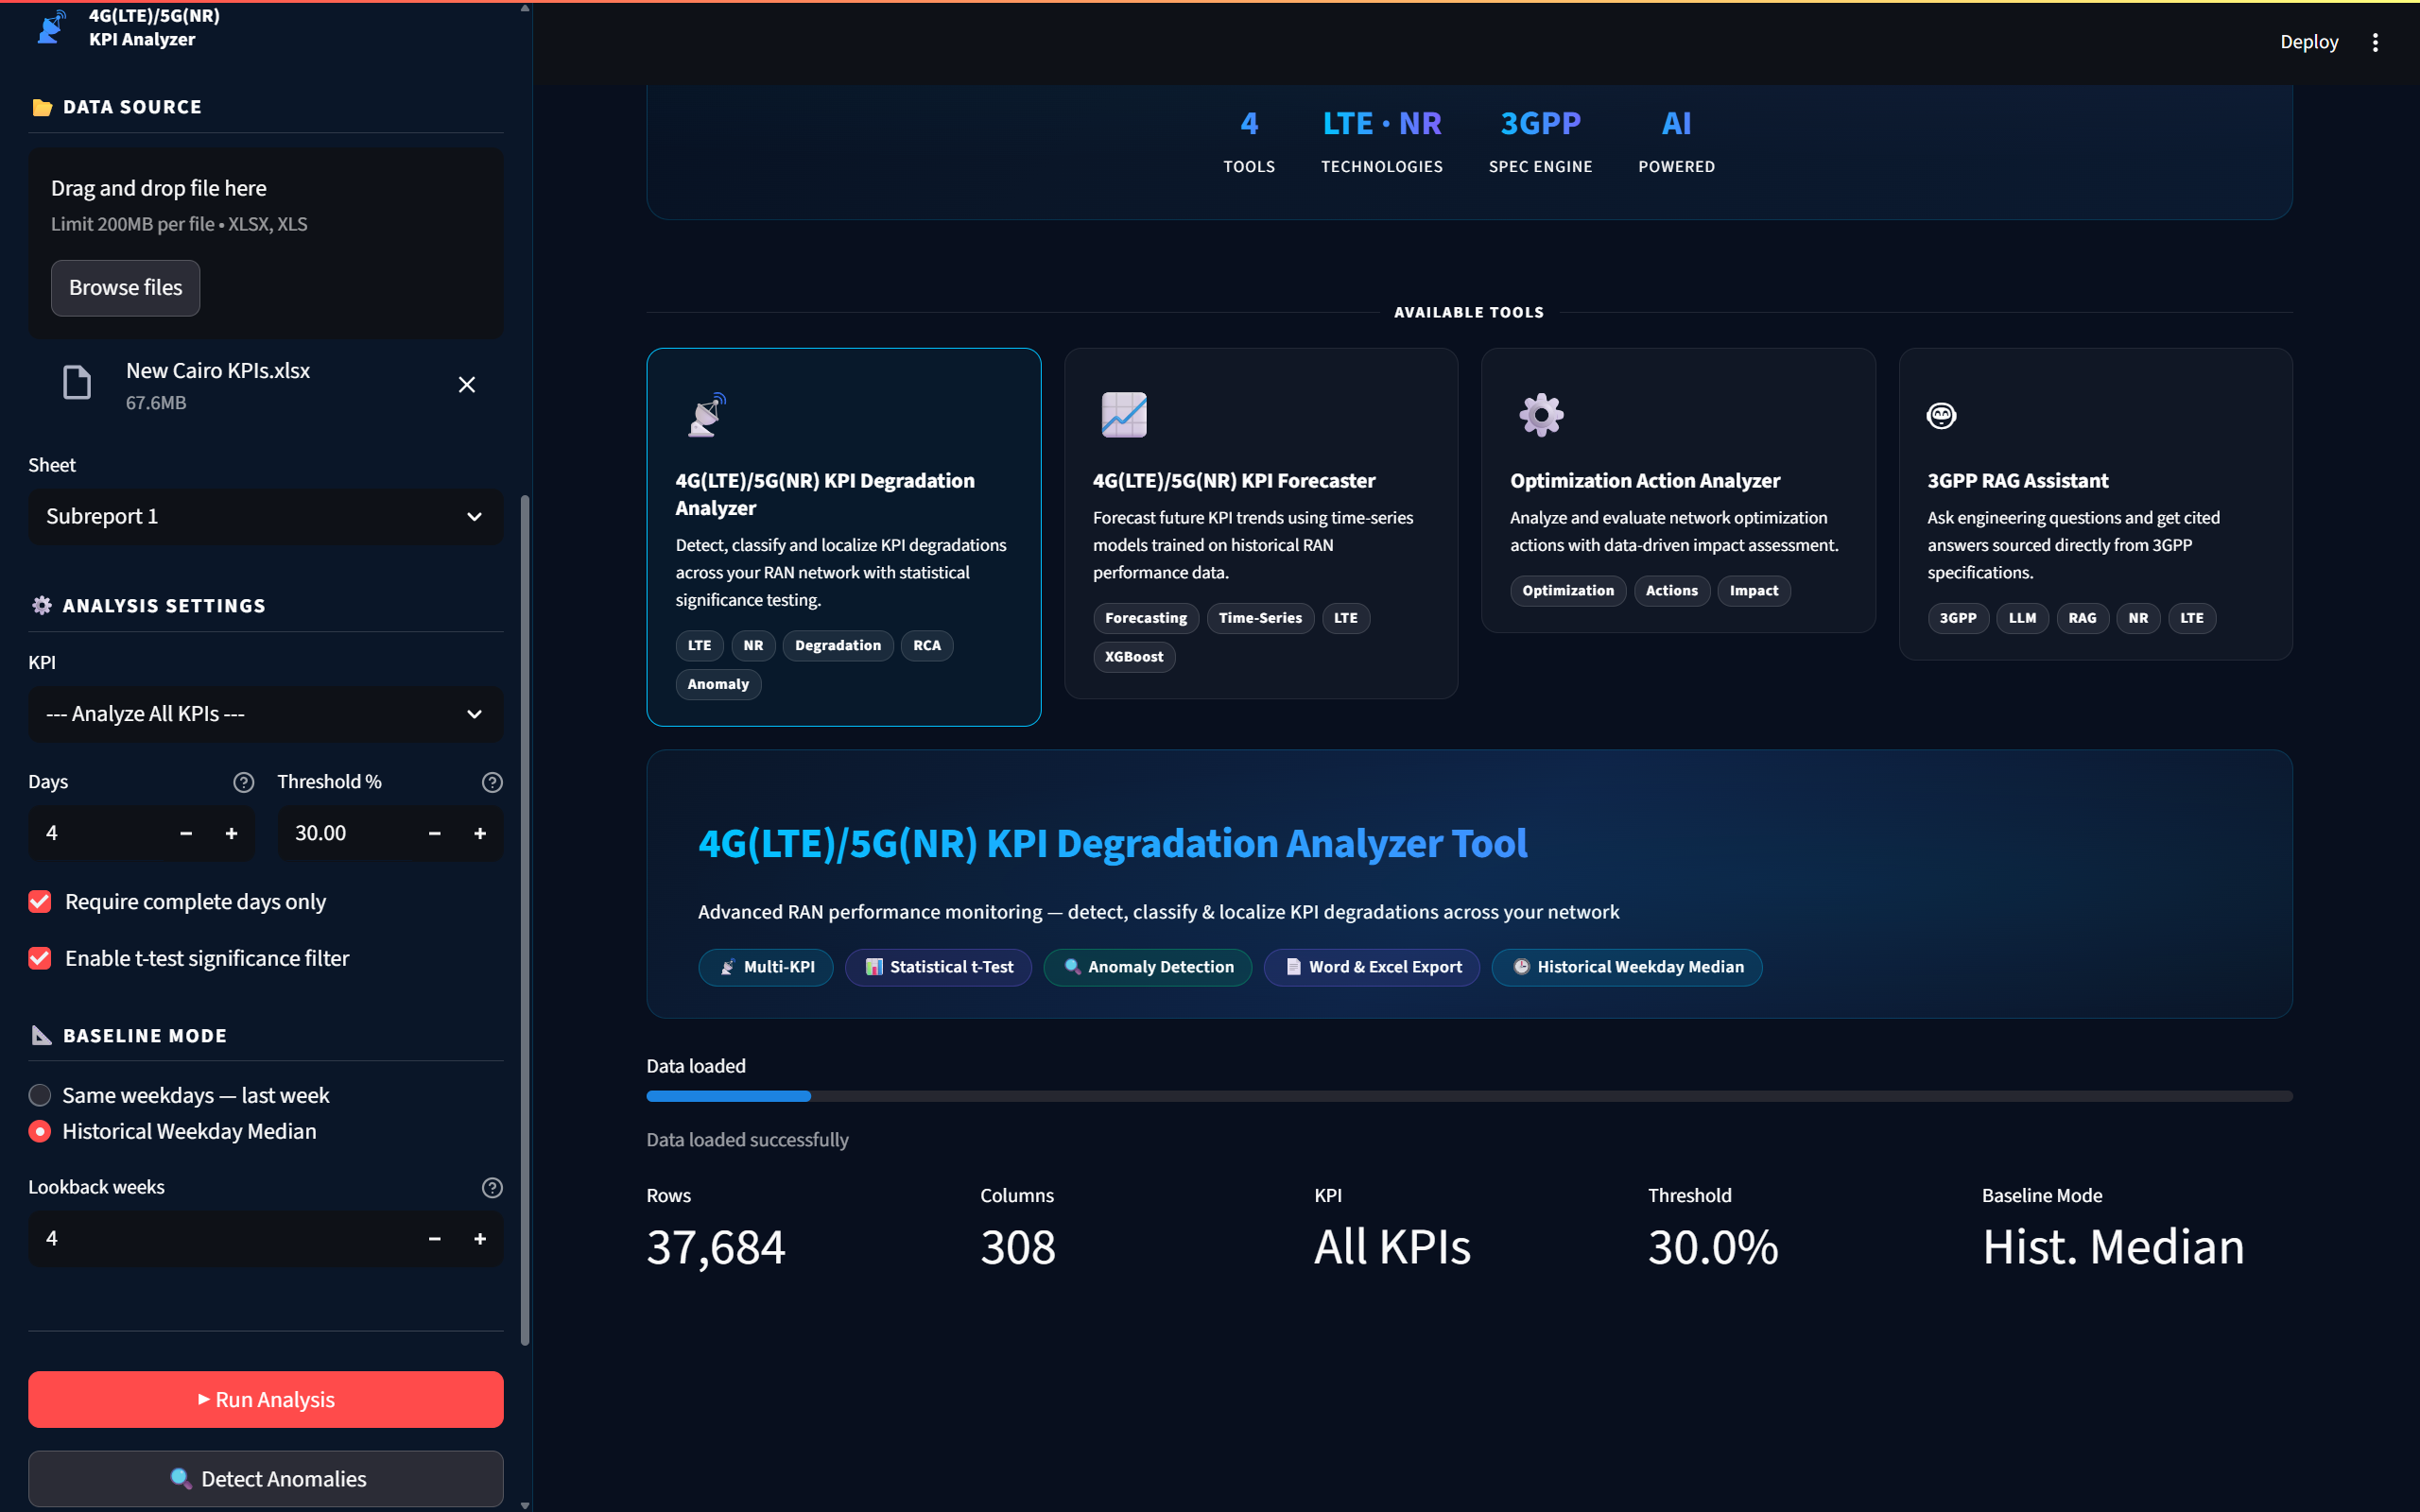
\includegraphics[width=\textwidth]{figures/chapter04/analysis_configuration.png}
    \caption{KPI Degradation Analyzer configuration panel after loading the New Cairo KPI dataset (37{,}684 rows, 308 columns). The sidebar shows the selected analysis settings: All KPIs, 4-day observation window, 30\% degradation threshold, Historical Weekday Median baseline mode, and 4 lookback weeks.}
    \label{fig:analysis_configuration}
\end{figure}

The configurable analysis parameters are as follows:

\begin{itemize}
    \item \textbf{KPI selection}: Engineers can choose to analyse all supported KPI categories simultaneously or restrict analysis to a specific KPI category.

    \item \textbf{Observation window}: The number of days in the recent observation window used for comparison against the baseline. A shorter window detects acute degradations while a longer window provides more stable statistical estimates.

    \item \textbf{Degradation threshold}: The minimum percentage degradation magnitude required to classify a cell-KPI combination as degraded. The default threshold of 30\% balances detection sensitivity against false positive rate.

    \item \textbf{Complete days filter}: When enabled, cells with incomplete observation records for the specified window are excluded from analysis to prevent artefactual degradation detection due to missing data.

    \item \textbf{t-test significance filter}: When enabled, the Welch's t-test p-value is applied as an additional filter, retaining only degradations that pass a specified significance threshold.

    \item \textbf{Baseline mode}: Engineers select between two baseline computation methods. \emph{Same Weekdays -- Last Week} computes the baseline from the corresponding weekday in the immediately preceding week, providing sensitivity to acute changes. \emph{Historical Weekday Median} computes the baseline from the median of the same weekday across the most recent $N$ weeks (configurable via the lookback weeks parameter), providing a more stable long-term baseline that is robust to week-to-week variability.
\end{itemize}

%%%%%%%%%%%%%%%%%%%%%%%%%%%%%%%%%%%%%%%%%%%%%%%%%%%%%%%%%%%%%%%%%%%%%%%%%%%%%%%%
\section{Analysis Results and KPI Summary}

Upon completion of the analysis pipeline, the module presents a structured summary of the detected degradations. Figure~\ref{fig:analysis_summary} shows the KPI Summary tab after a full analysis of the New Cairo dataset, which identified 784 total degraded cells across 13 KPI categories.

\begin{figure}[H]
    \centering
    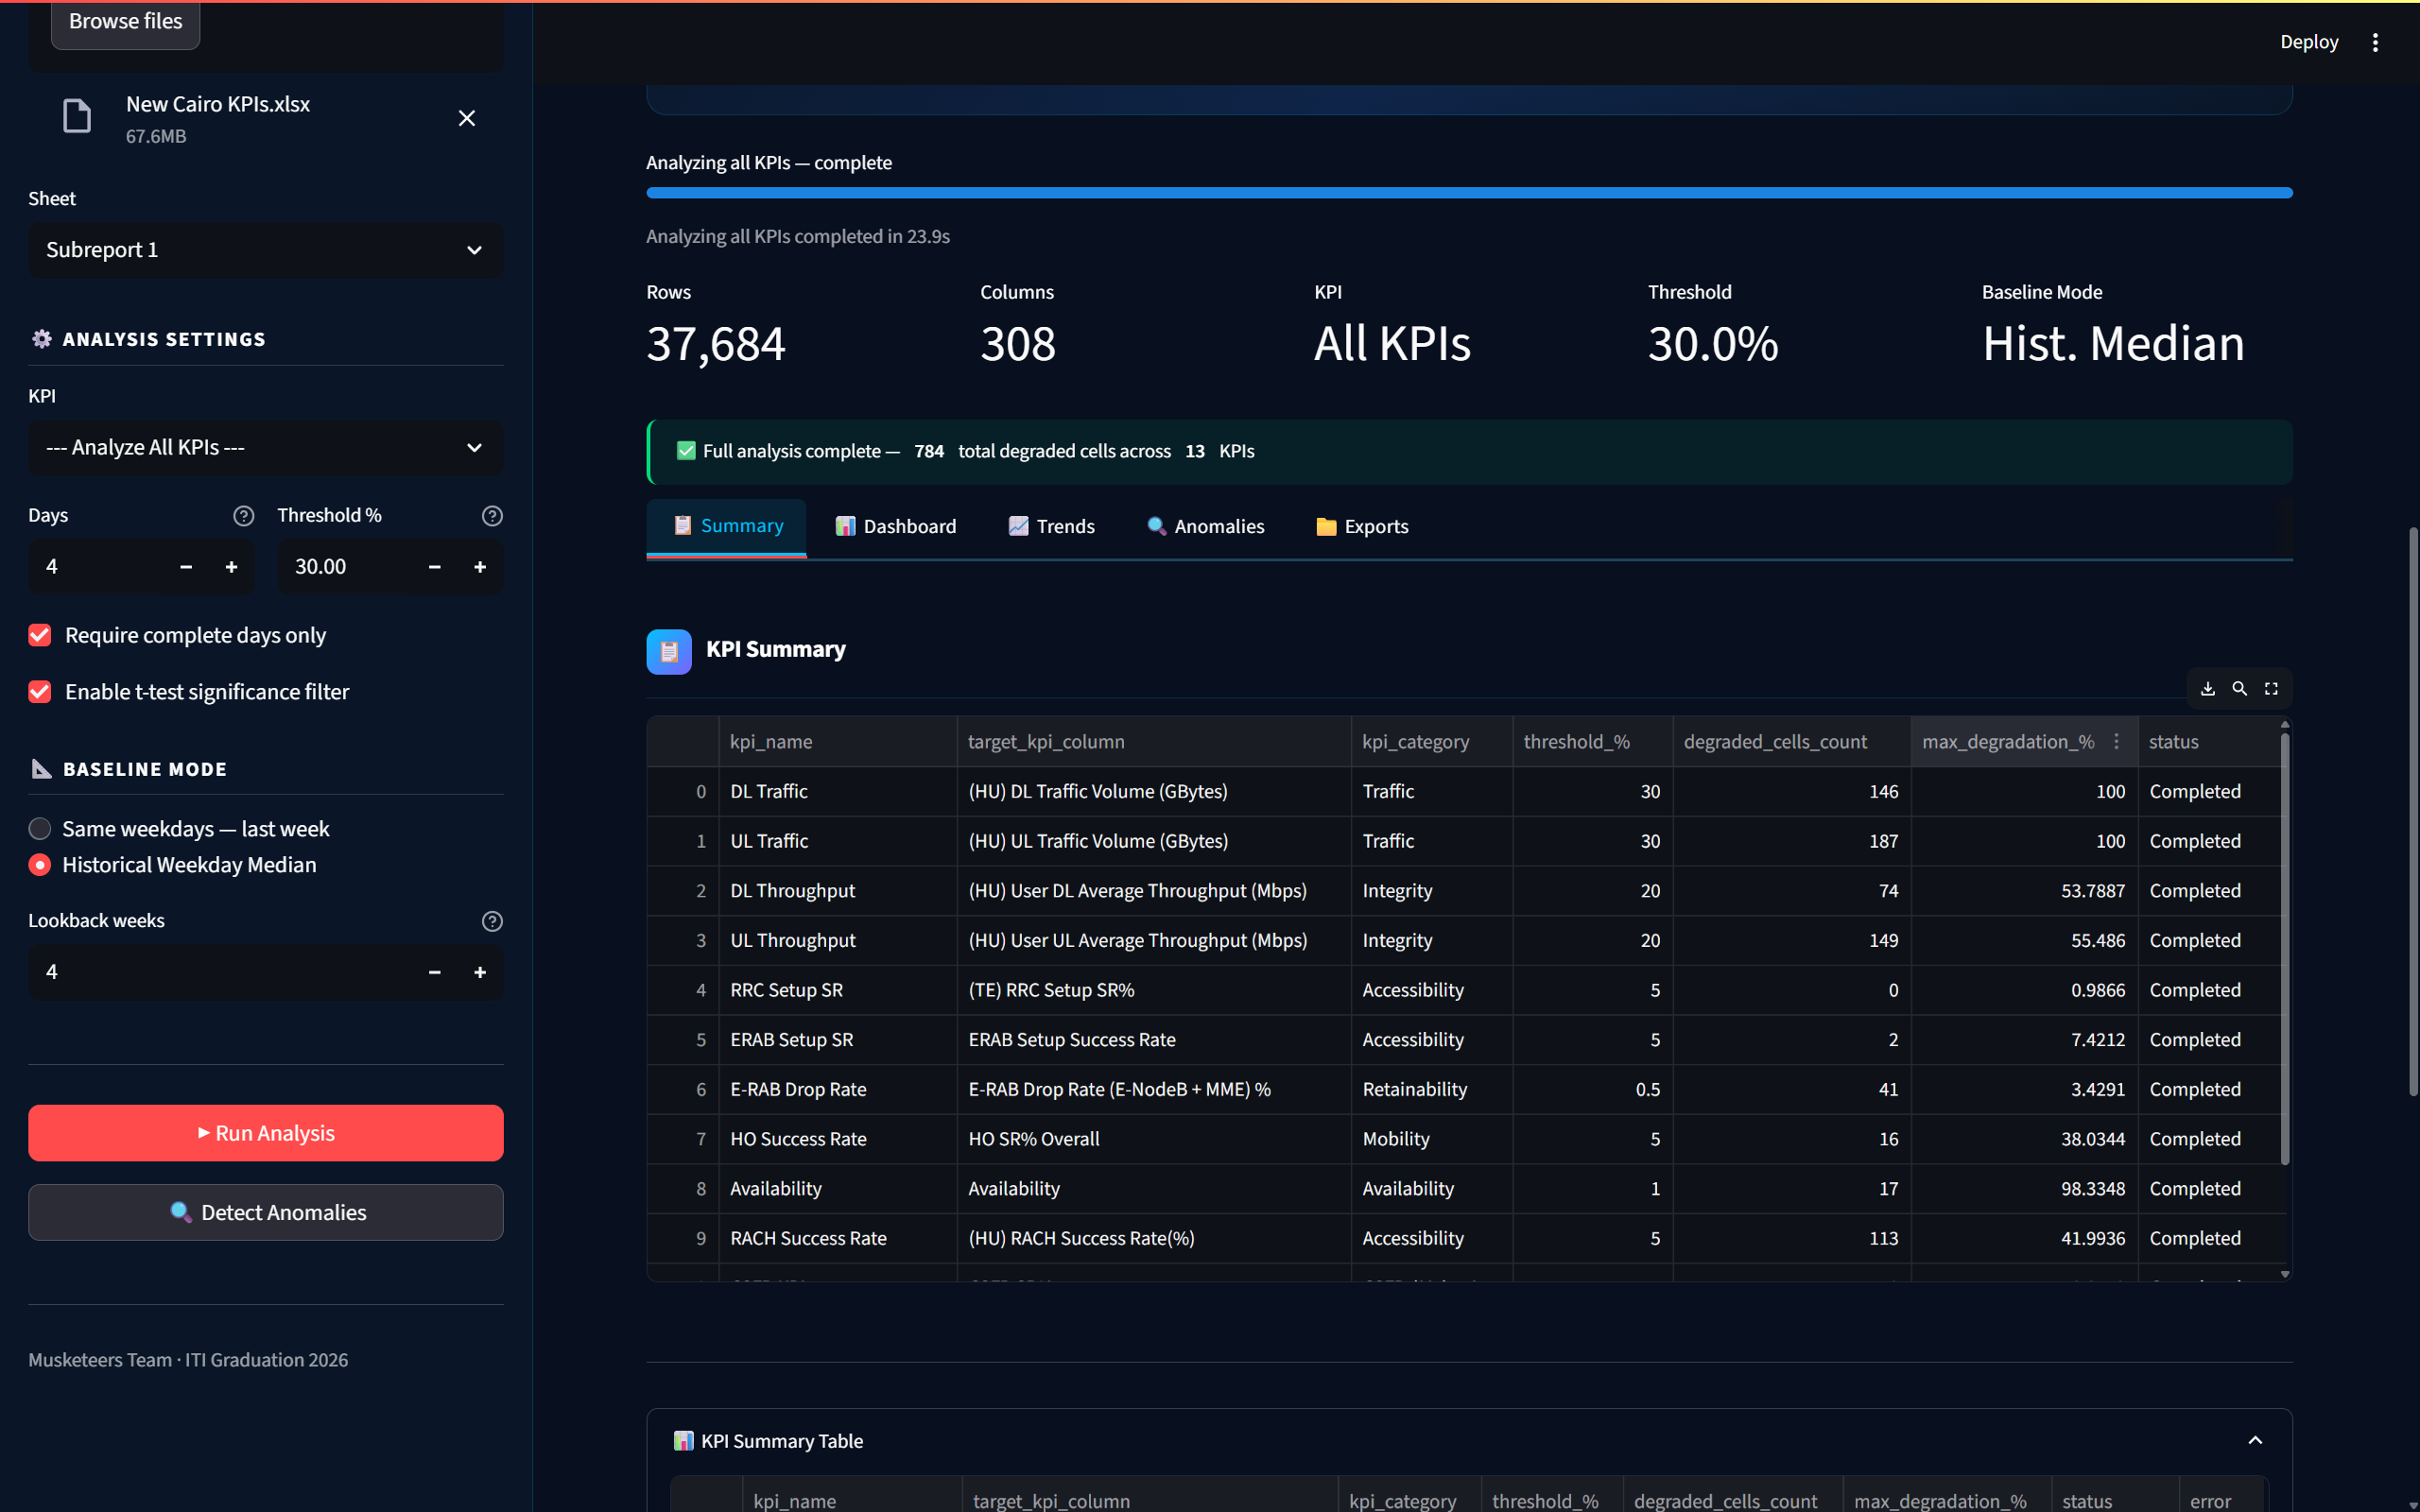
\includegraphics[width=\textwidth]{figures/chapter04/analysis_summary.png}
    \caption{KPI Summary tab showing the analysis results for the New Cairo dataset (37{,}684 rows, 308 columns, All KPIs, 30\% threshold, Historical Weekday Median baseline). The table lists each KPI category with its degraded cell count and maximum degradation percentage.}
    \label{fig:analysis_summary}
\end{figure}

The KPI Summary table presents each monitored KPI category with the following fields:

\begin{itemize}
    \item \textbf{kpi\_name}: The human-readable name of the KPI category.
    \item \textbf{target\_kpi\_column}: The specific counter column name used for degradation computation.
    \item \textbf{kpi\_category}: The performance pillar classification (Traffic, Integrity, Accessibility, Retainability, Mobility, Availability).
    \item \textbf{threshold\_\%}: The degradation threshold applied to this KPI category.
    \item \textbf{degraded\_cells\_count}: The number of cells classified as degraded for this KPI.
    \item \textbf{max\_degradation\_\%}: The maximum observed degradation percentage across all degraded cells for this KPI.
    \item \textbf{status}: Completion status of the analysis for this KPI (Completed or Error).
\end{itemize}

%%%%%%%%%%%%%%%%%%%%%%%%%%%%%%%%%%%%%%%%%%%%%%%%%%%%%%%%%%%%%%%%%%%%%%%%%%%%%%%%
\section{Main Dashboard and Charts}

The Dashboard tab presents an aggregated visual summary of the degradation analysis results. Figure~\ref{fig:main_dashboard} illustrates the main dashboard view.

\begin{figure}[H]
    \centering
    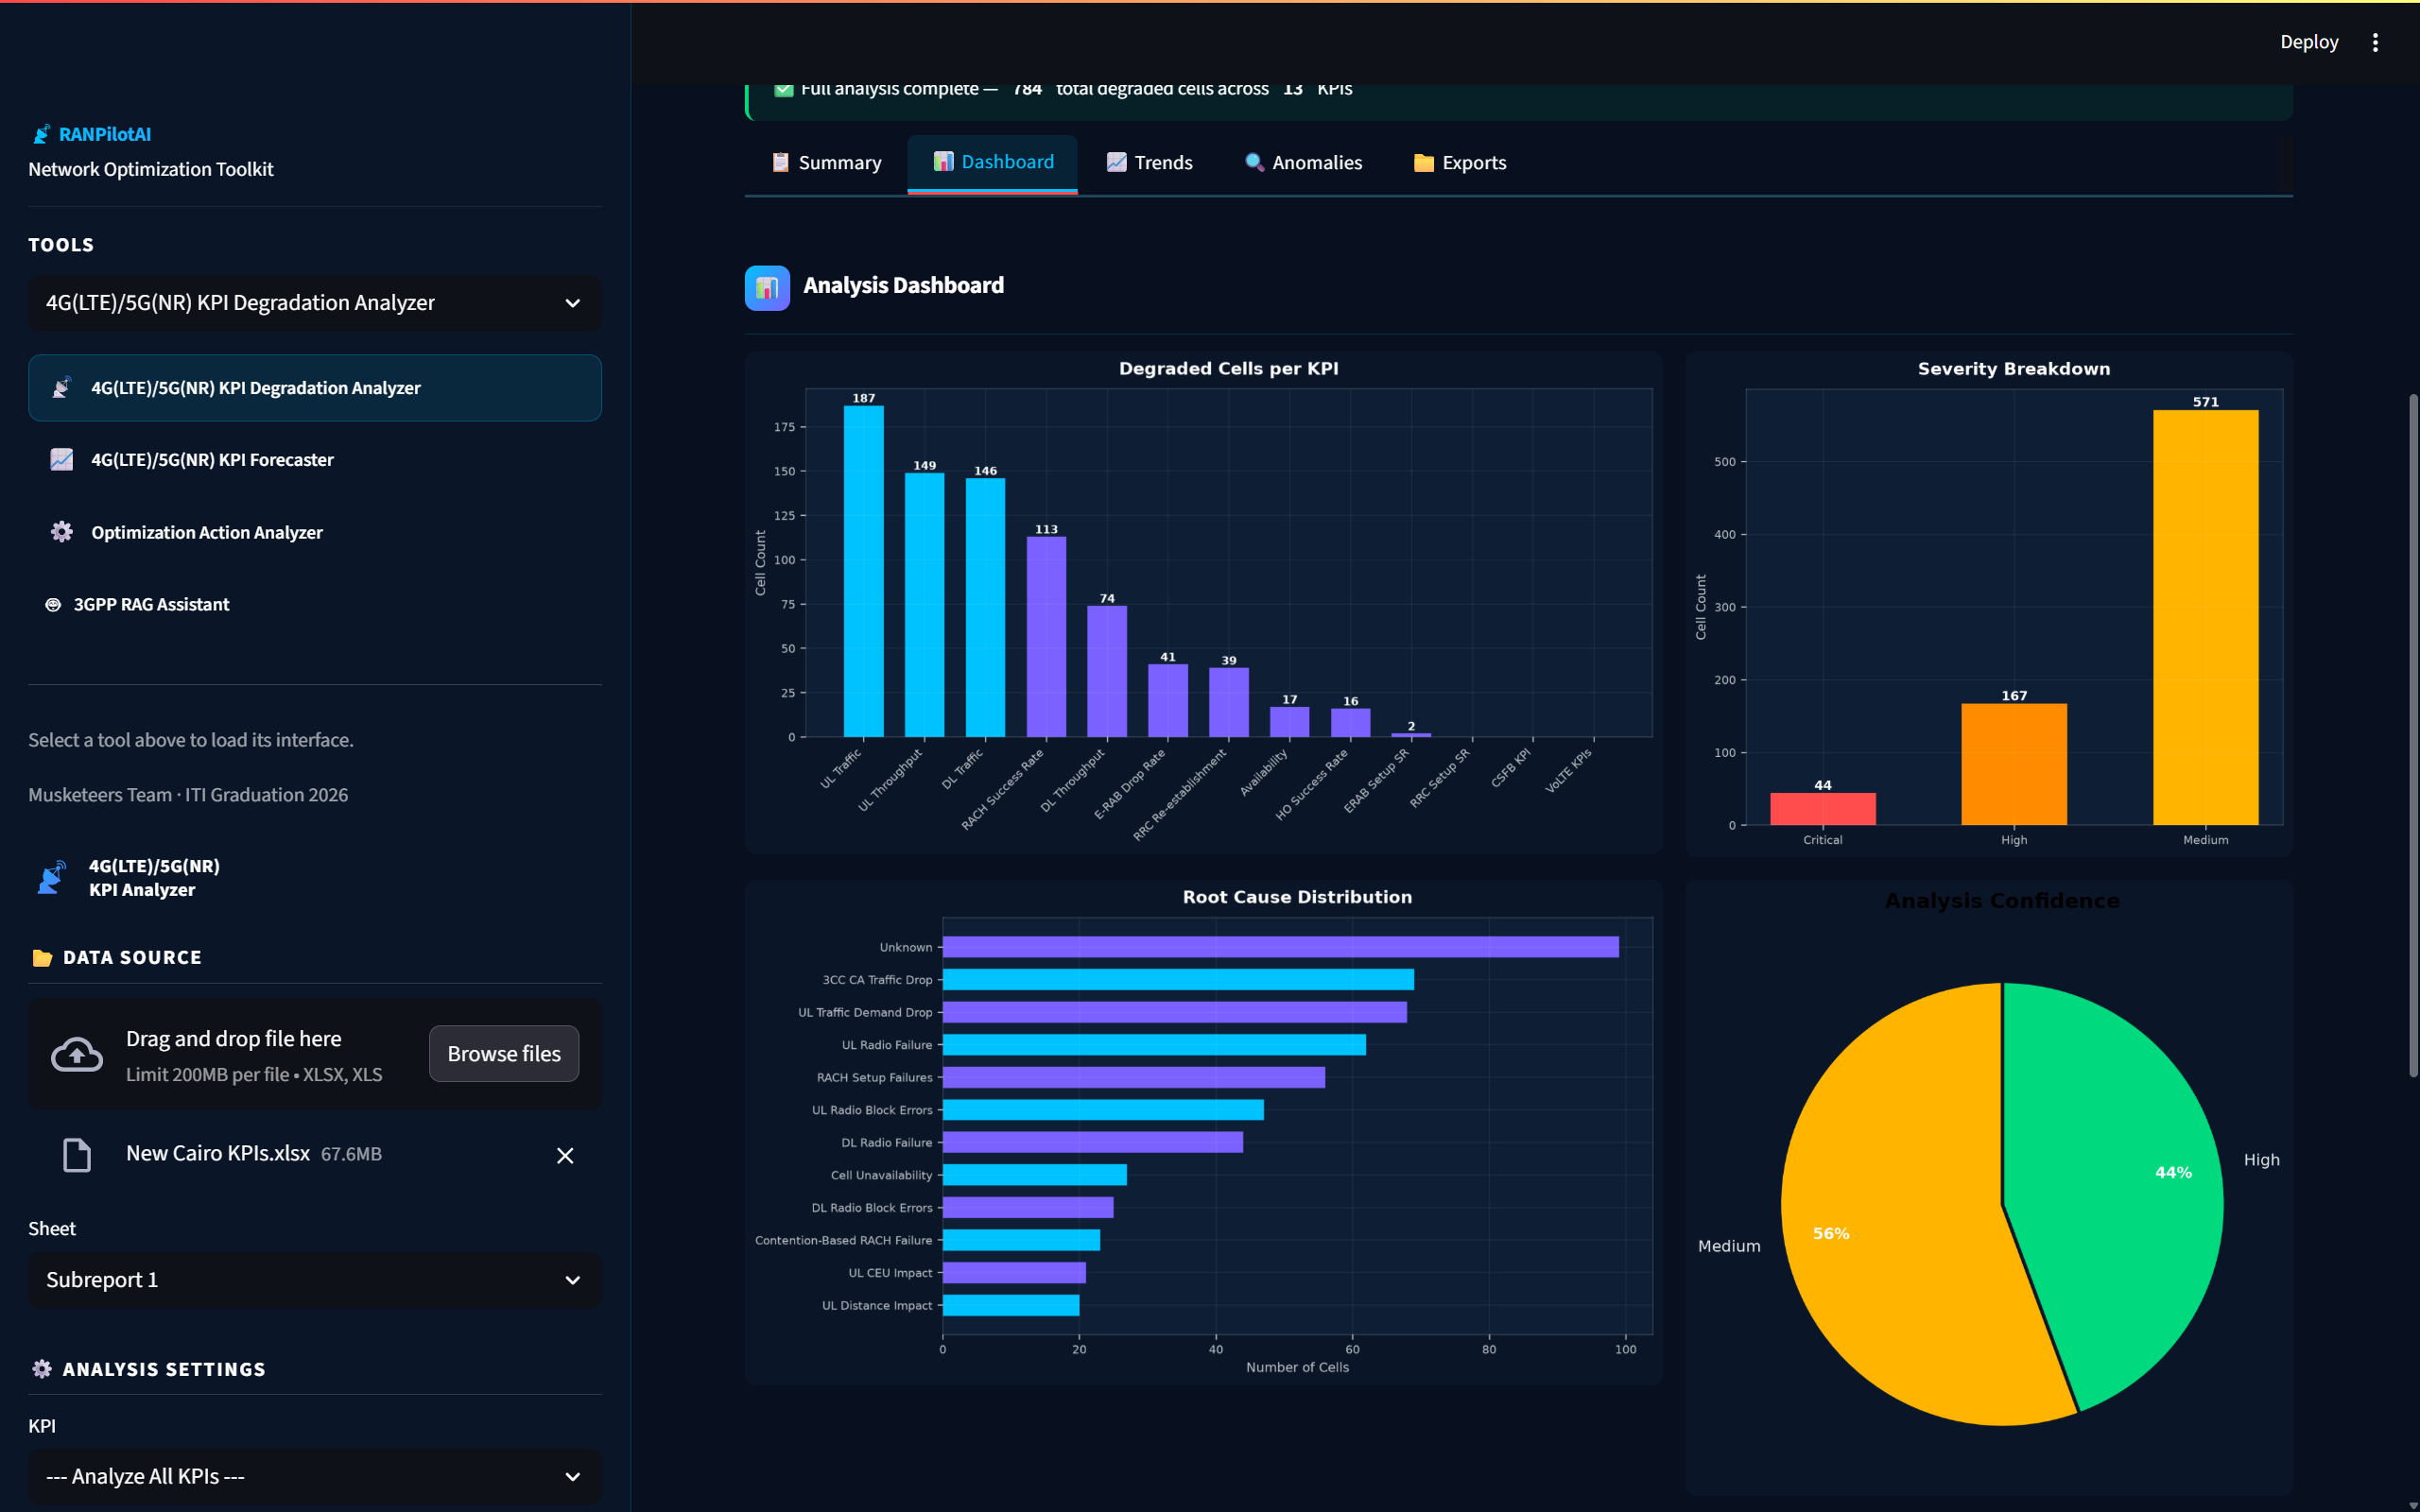
\includegraphics[width=\textwidth]{figures/chapter04/main_dashboard.png}
    \caption{KPI Degradation Analyzer main dashboard presenting KPI-level degradation metrics, cell count distributions, and interactive charts for the New Cairo dataset analysis.}
    \label{fig:main_dashboard}
\end{figure}

The dashboard provides multiple interactive chart types including:

\begin{itemize}
    \item KPI-level degraded cell count bar charts enabling engineers to identify which KPI categories are most severely affected.
    \item Degradation magnitude distribution histograms showing the distribution of degradation percentages across degraded cells.
    \item Root cause pattern distribution pie charts illustrating the relative frequency of different RCA classifications across all degraded cells.
    \item Confidence level distribution charts showing the proportion of High, Medium, and Low confidence degradation detections.
\end{itemize}

%%%%%%%%%%%%%%%%%%%%%%%%%%%%%%%%%%%%%%%%%%%%%%%%%%%%%%%%%%%%%%%%%%%%%%%%%%%%%%%%
\section{Root Cause Analysis}

\subsection{Root Cause Dashboard}

The root cause analysis output is presented through dedicated visualisation panels that enable engineers to drill down into specific cells and examine the RCA evidence in detail. Figure~\ref{fig:root_cause_dashboard} presents the root cause analysis dashboard.

\begin{figure}[H]
    \centering
    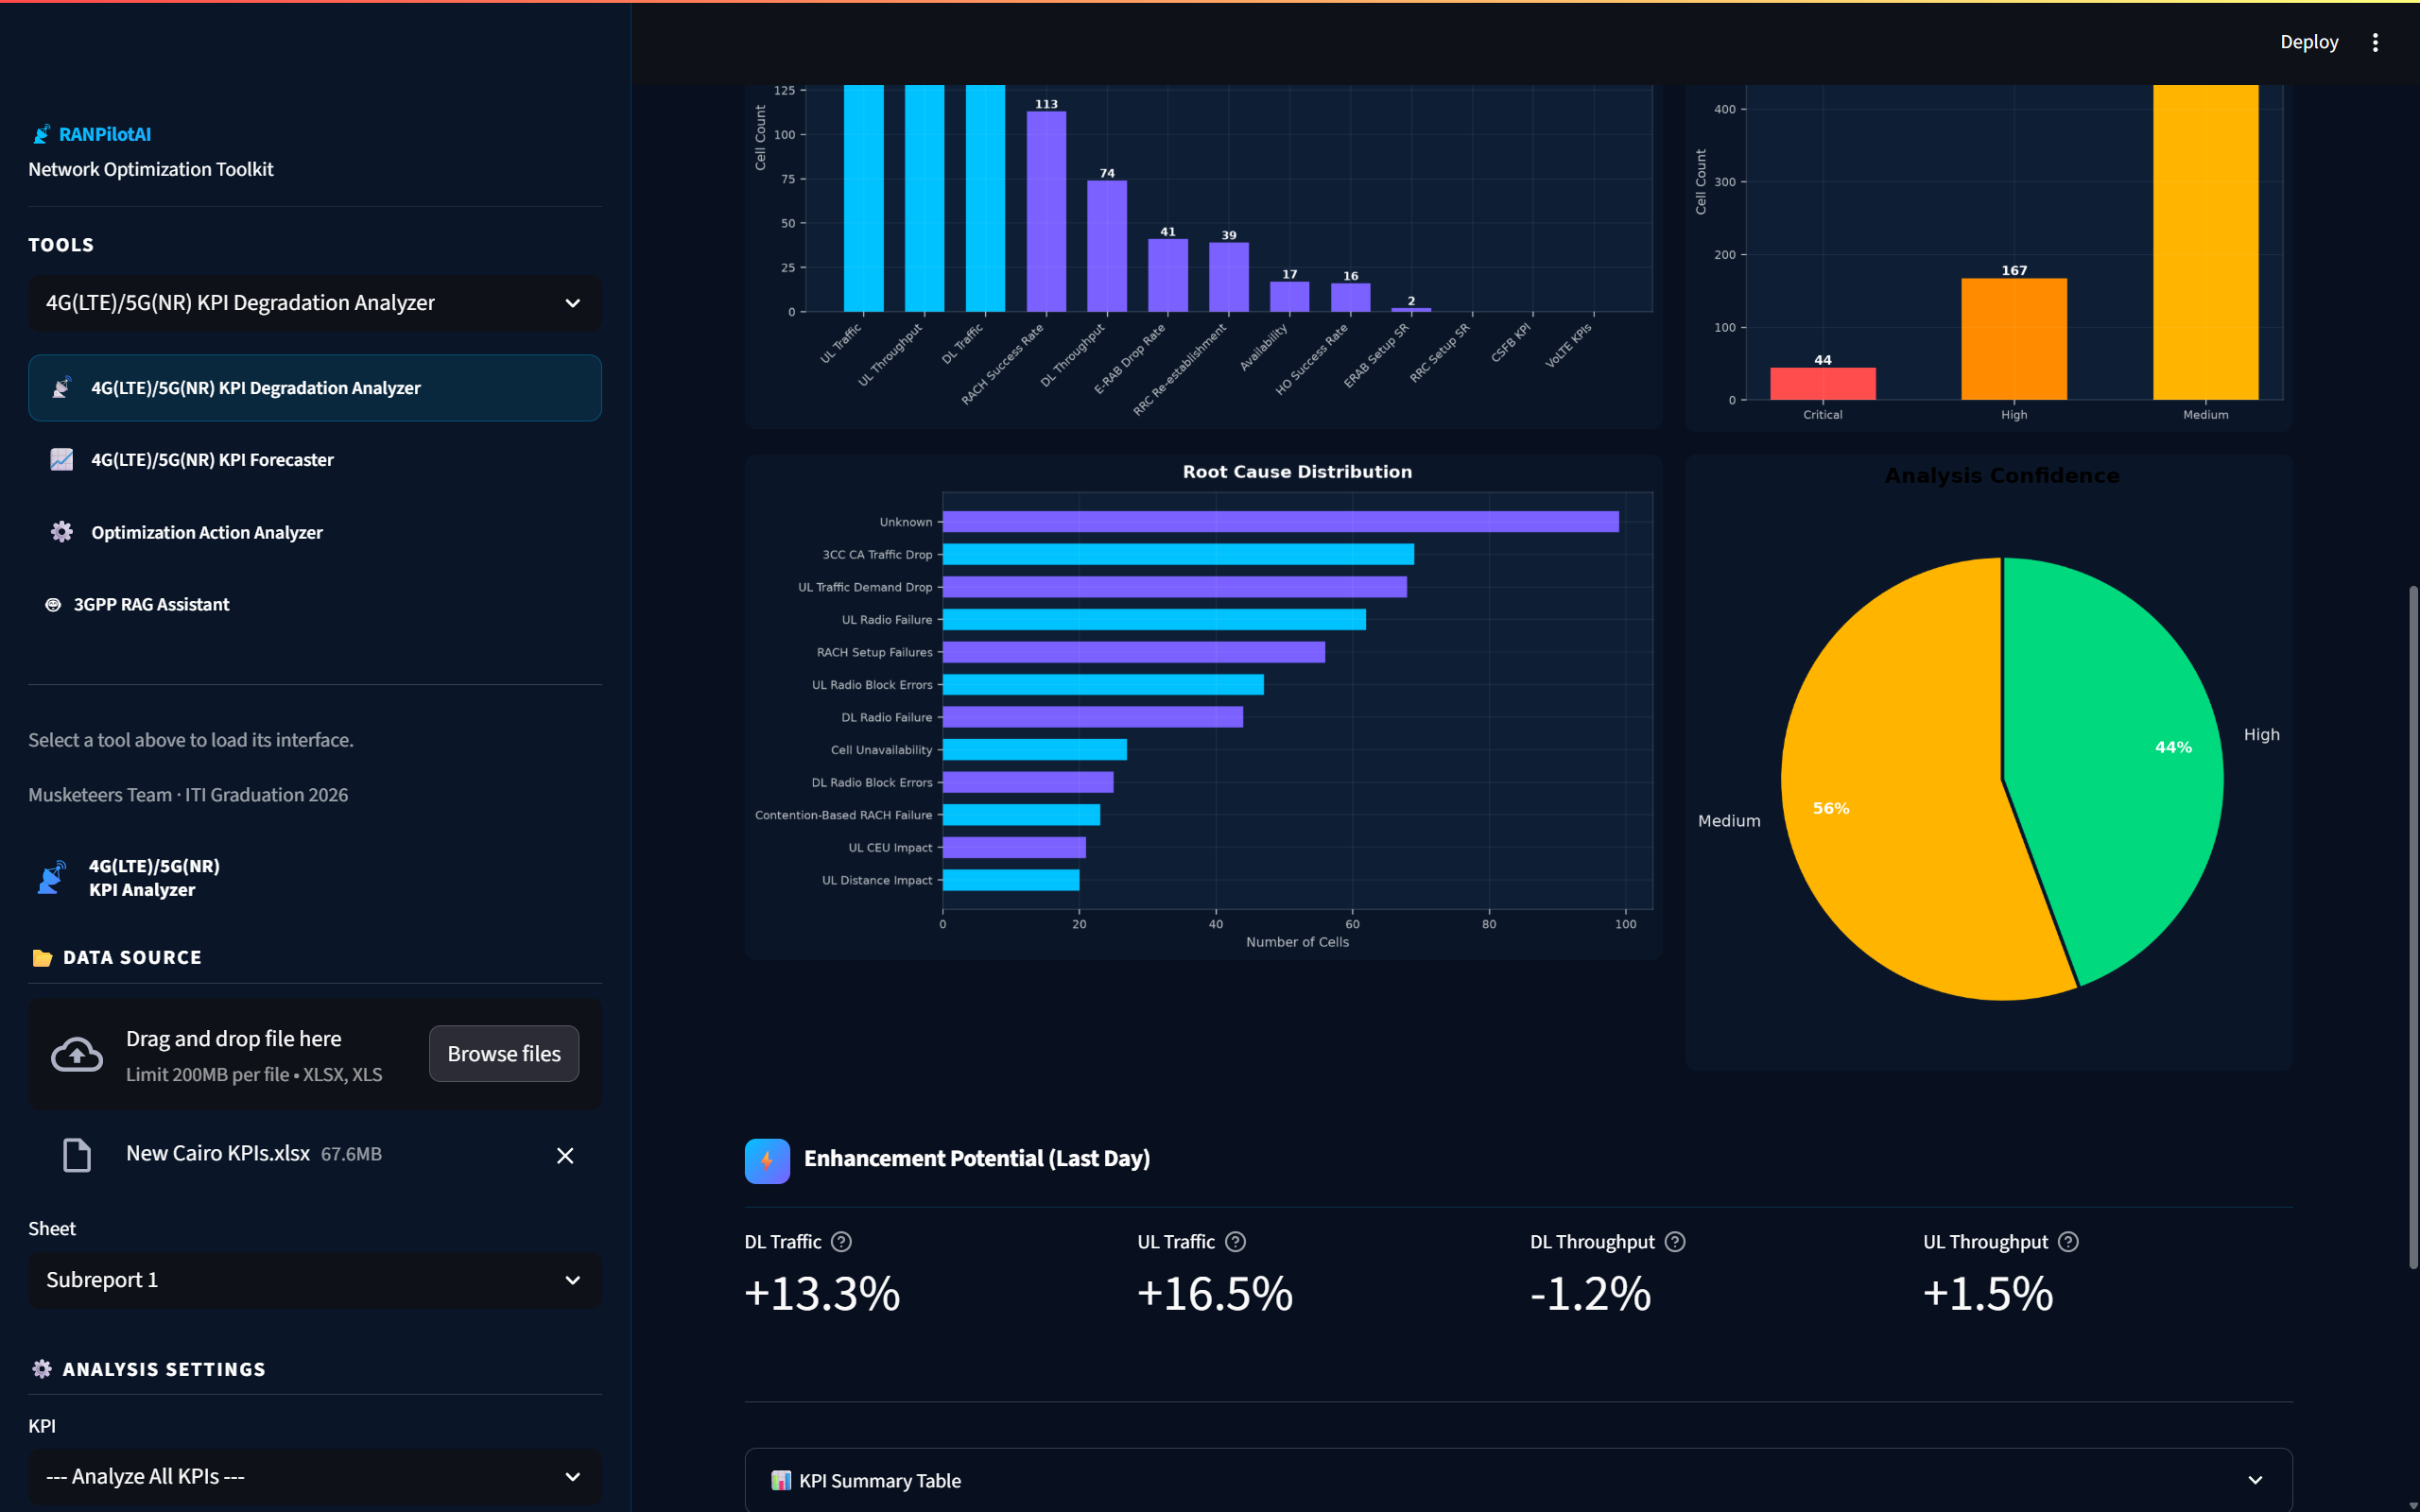
\includegraphics[width=\textwidth]{figures/chapter04/root_cause_dashboard.png}
    \caption{Root cause analysis dashboard showing the distribution of RCA pattern classifications, severity scores, and correlated diagnostic counter evidence across degraded cells in the New Cairo dataset.}
    \label{fig:root_cause_dashboard}
\end{figure}

\subsection{Root Cause Recommendations}

For each degraded cell, the RCA engine generates a structured recommendation that includes the primary root cause pattern, the supporting diagnostic evidence, and a set of recommended next investigation steps. Figure~\ref{fig:root_cause_recommendation} illustrates the root cause recommendation output for a representative degraded cell.

\begin{figure}[H]
    \centering
    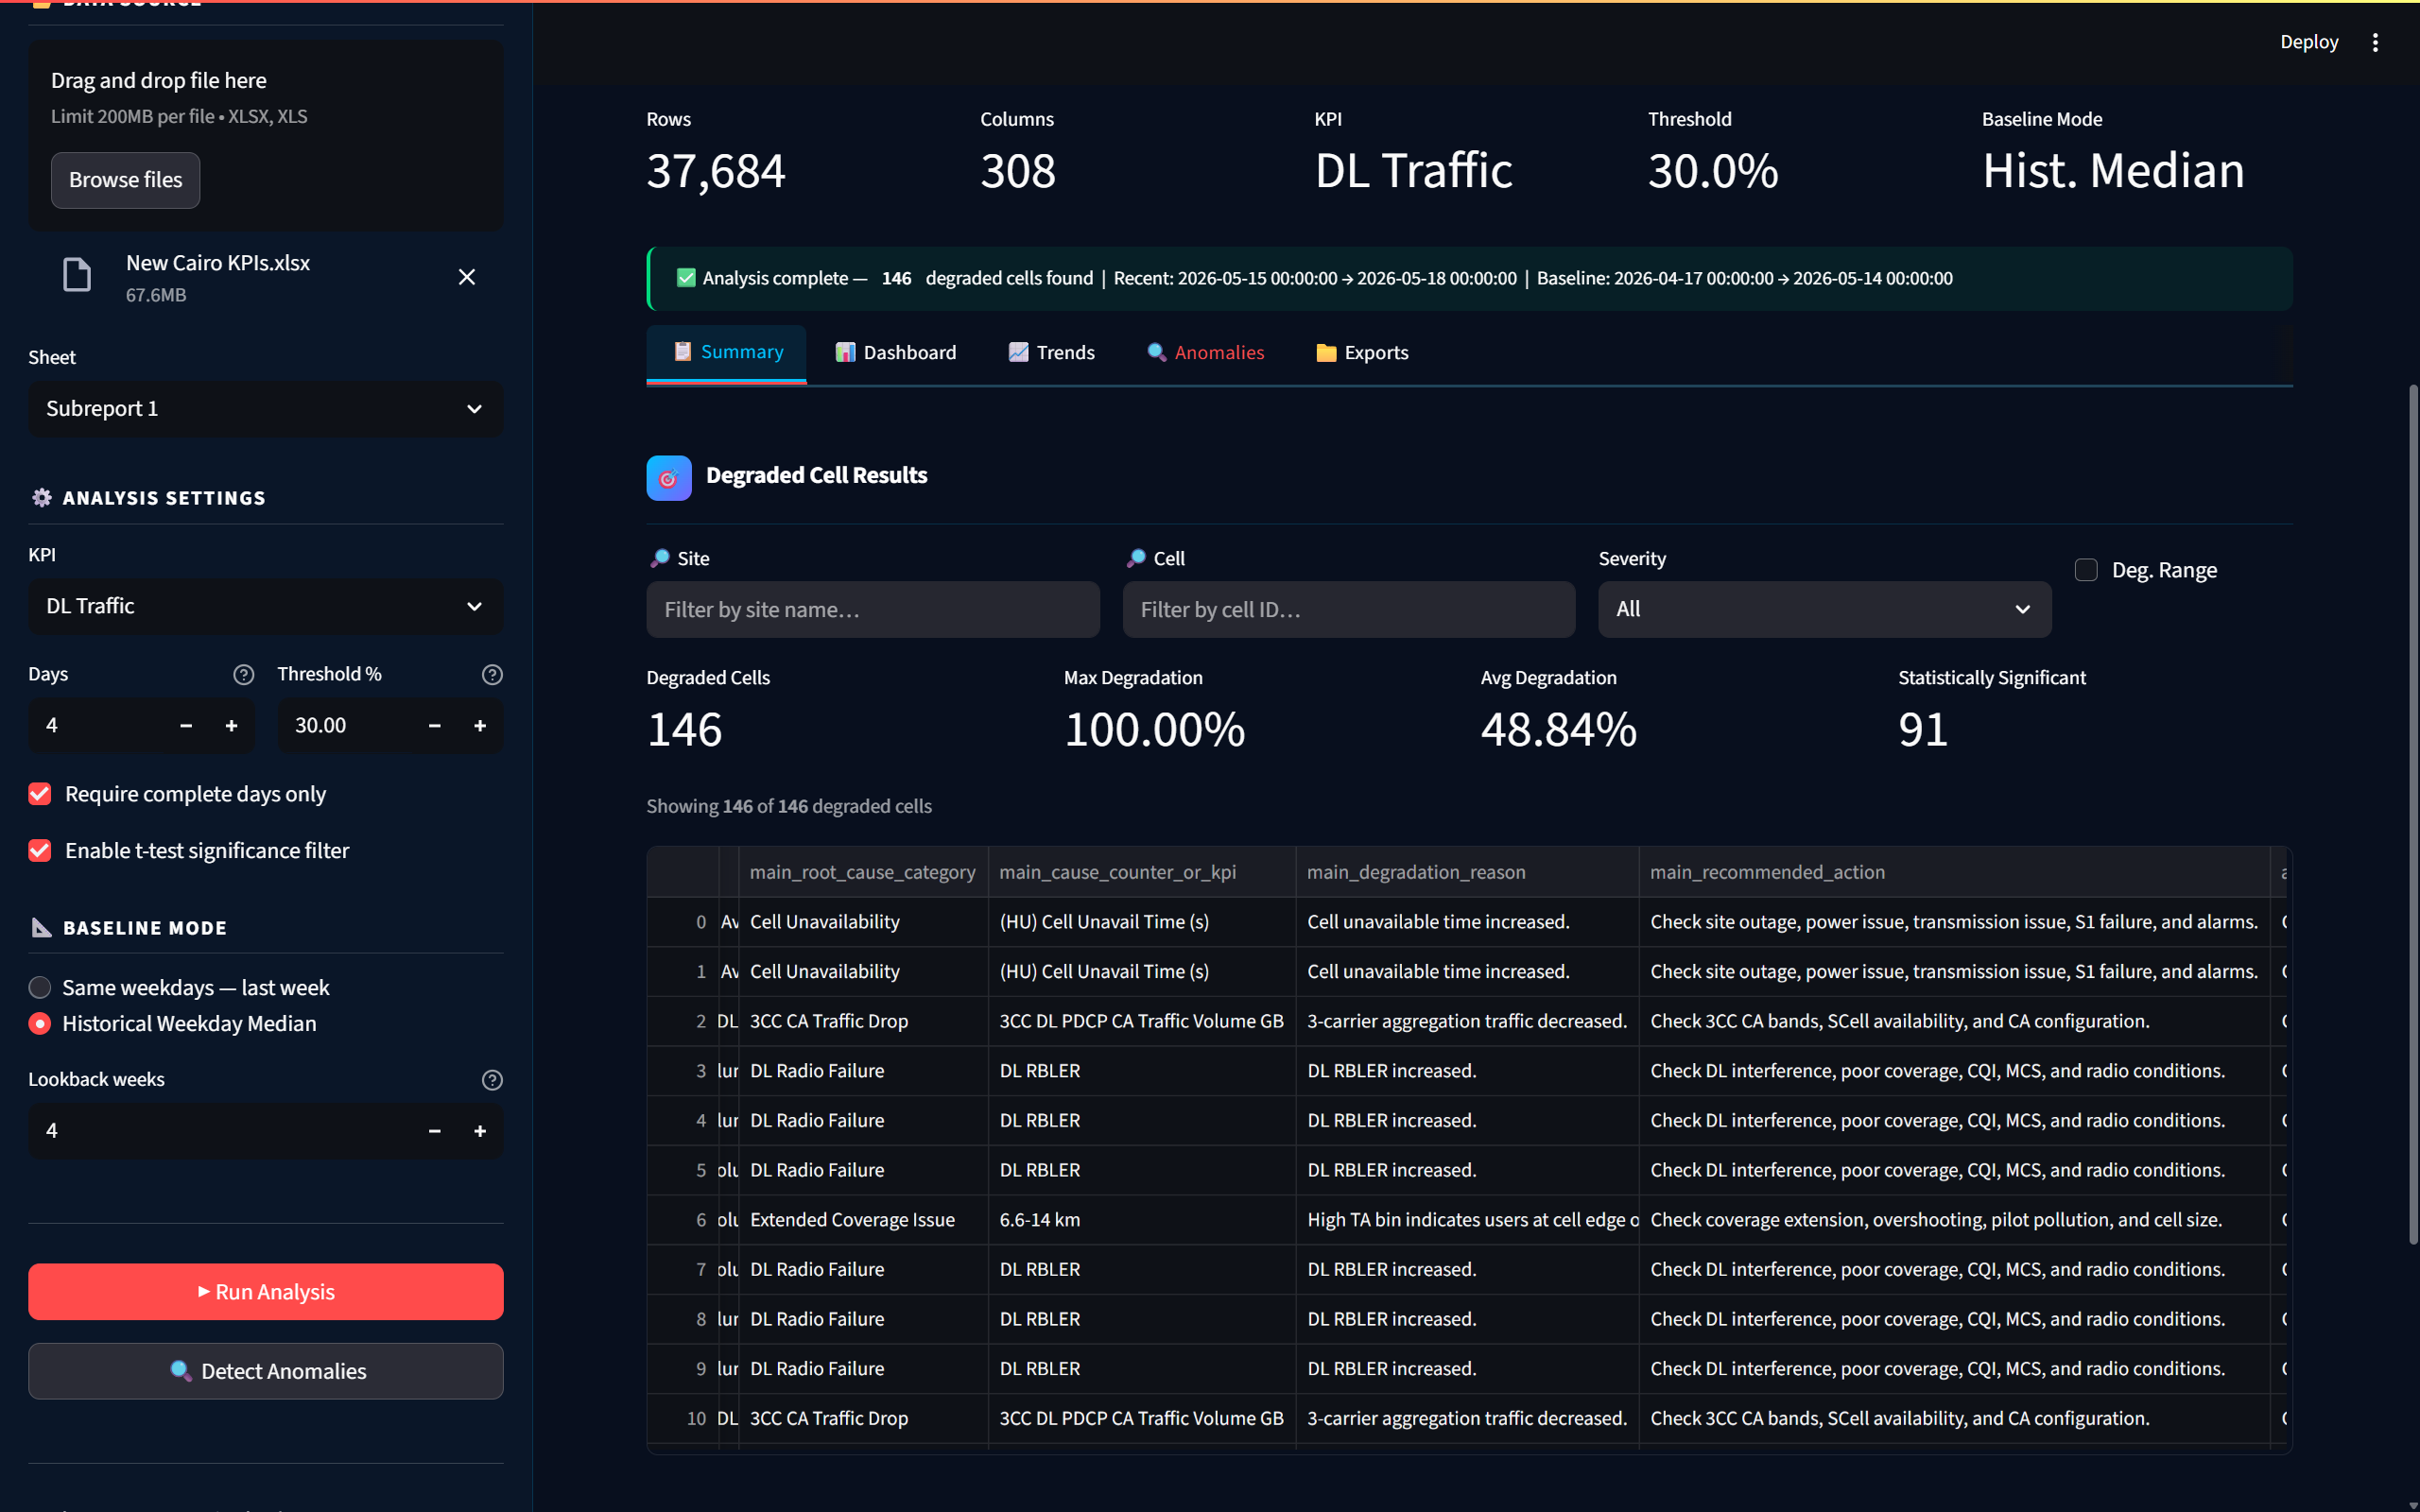
\includegraphics[width=\textwidth]{figures/chapter04/root_cause_recommendation.png}
    \caption{Root cause recommendation panel for a degraded cell, showing the identified RCA pattern, supporting correlated counter evidence, RF severity classification, and recommended next investigation steps.}
    \label{fig:root_cause_recommendation}
\end{figure}

The root cause recommendation output includes the following structured fields:

\begin{itemize}
    \item \textbf{rca\_pattern}: The classified root cause pattern (Outage, Congestion, Radio Quality, Coverage, Interference, Mobility, Demand, or Unknown).
    \item \textbf{main\_root\_cause\_category}: A human-readable label for the primary root cause category.
    \item \textbf{rf\_severity}: A severity classification (Critical, High, Medium, or Low) based on the composite RCA score.
    \item \textbf{analysis\_confidence}: The statistical confidence level of the degradation detection (High, Medium, or Low).
    \item \textbf{confidence\_reason}: A textual explanation of the factors contributing to the assigned confidence level.
    \item \textbf{next\_investigation\_steps}: A list of specific counter values and diagnostic checks recommended for the engineer to perform as the next step in the troubleshooting workflow.
\end{itemize}

\subsection{Severity and Confidence Metrics}

Figure~\ref{fig:severity_confidence} presents the severity and confidence metric panels, which provide an aggregated view of the RCA output quality and the distribution of severity levels across all degraded cells.

\begin{figure}[H]
    \centering
    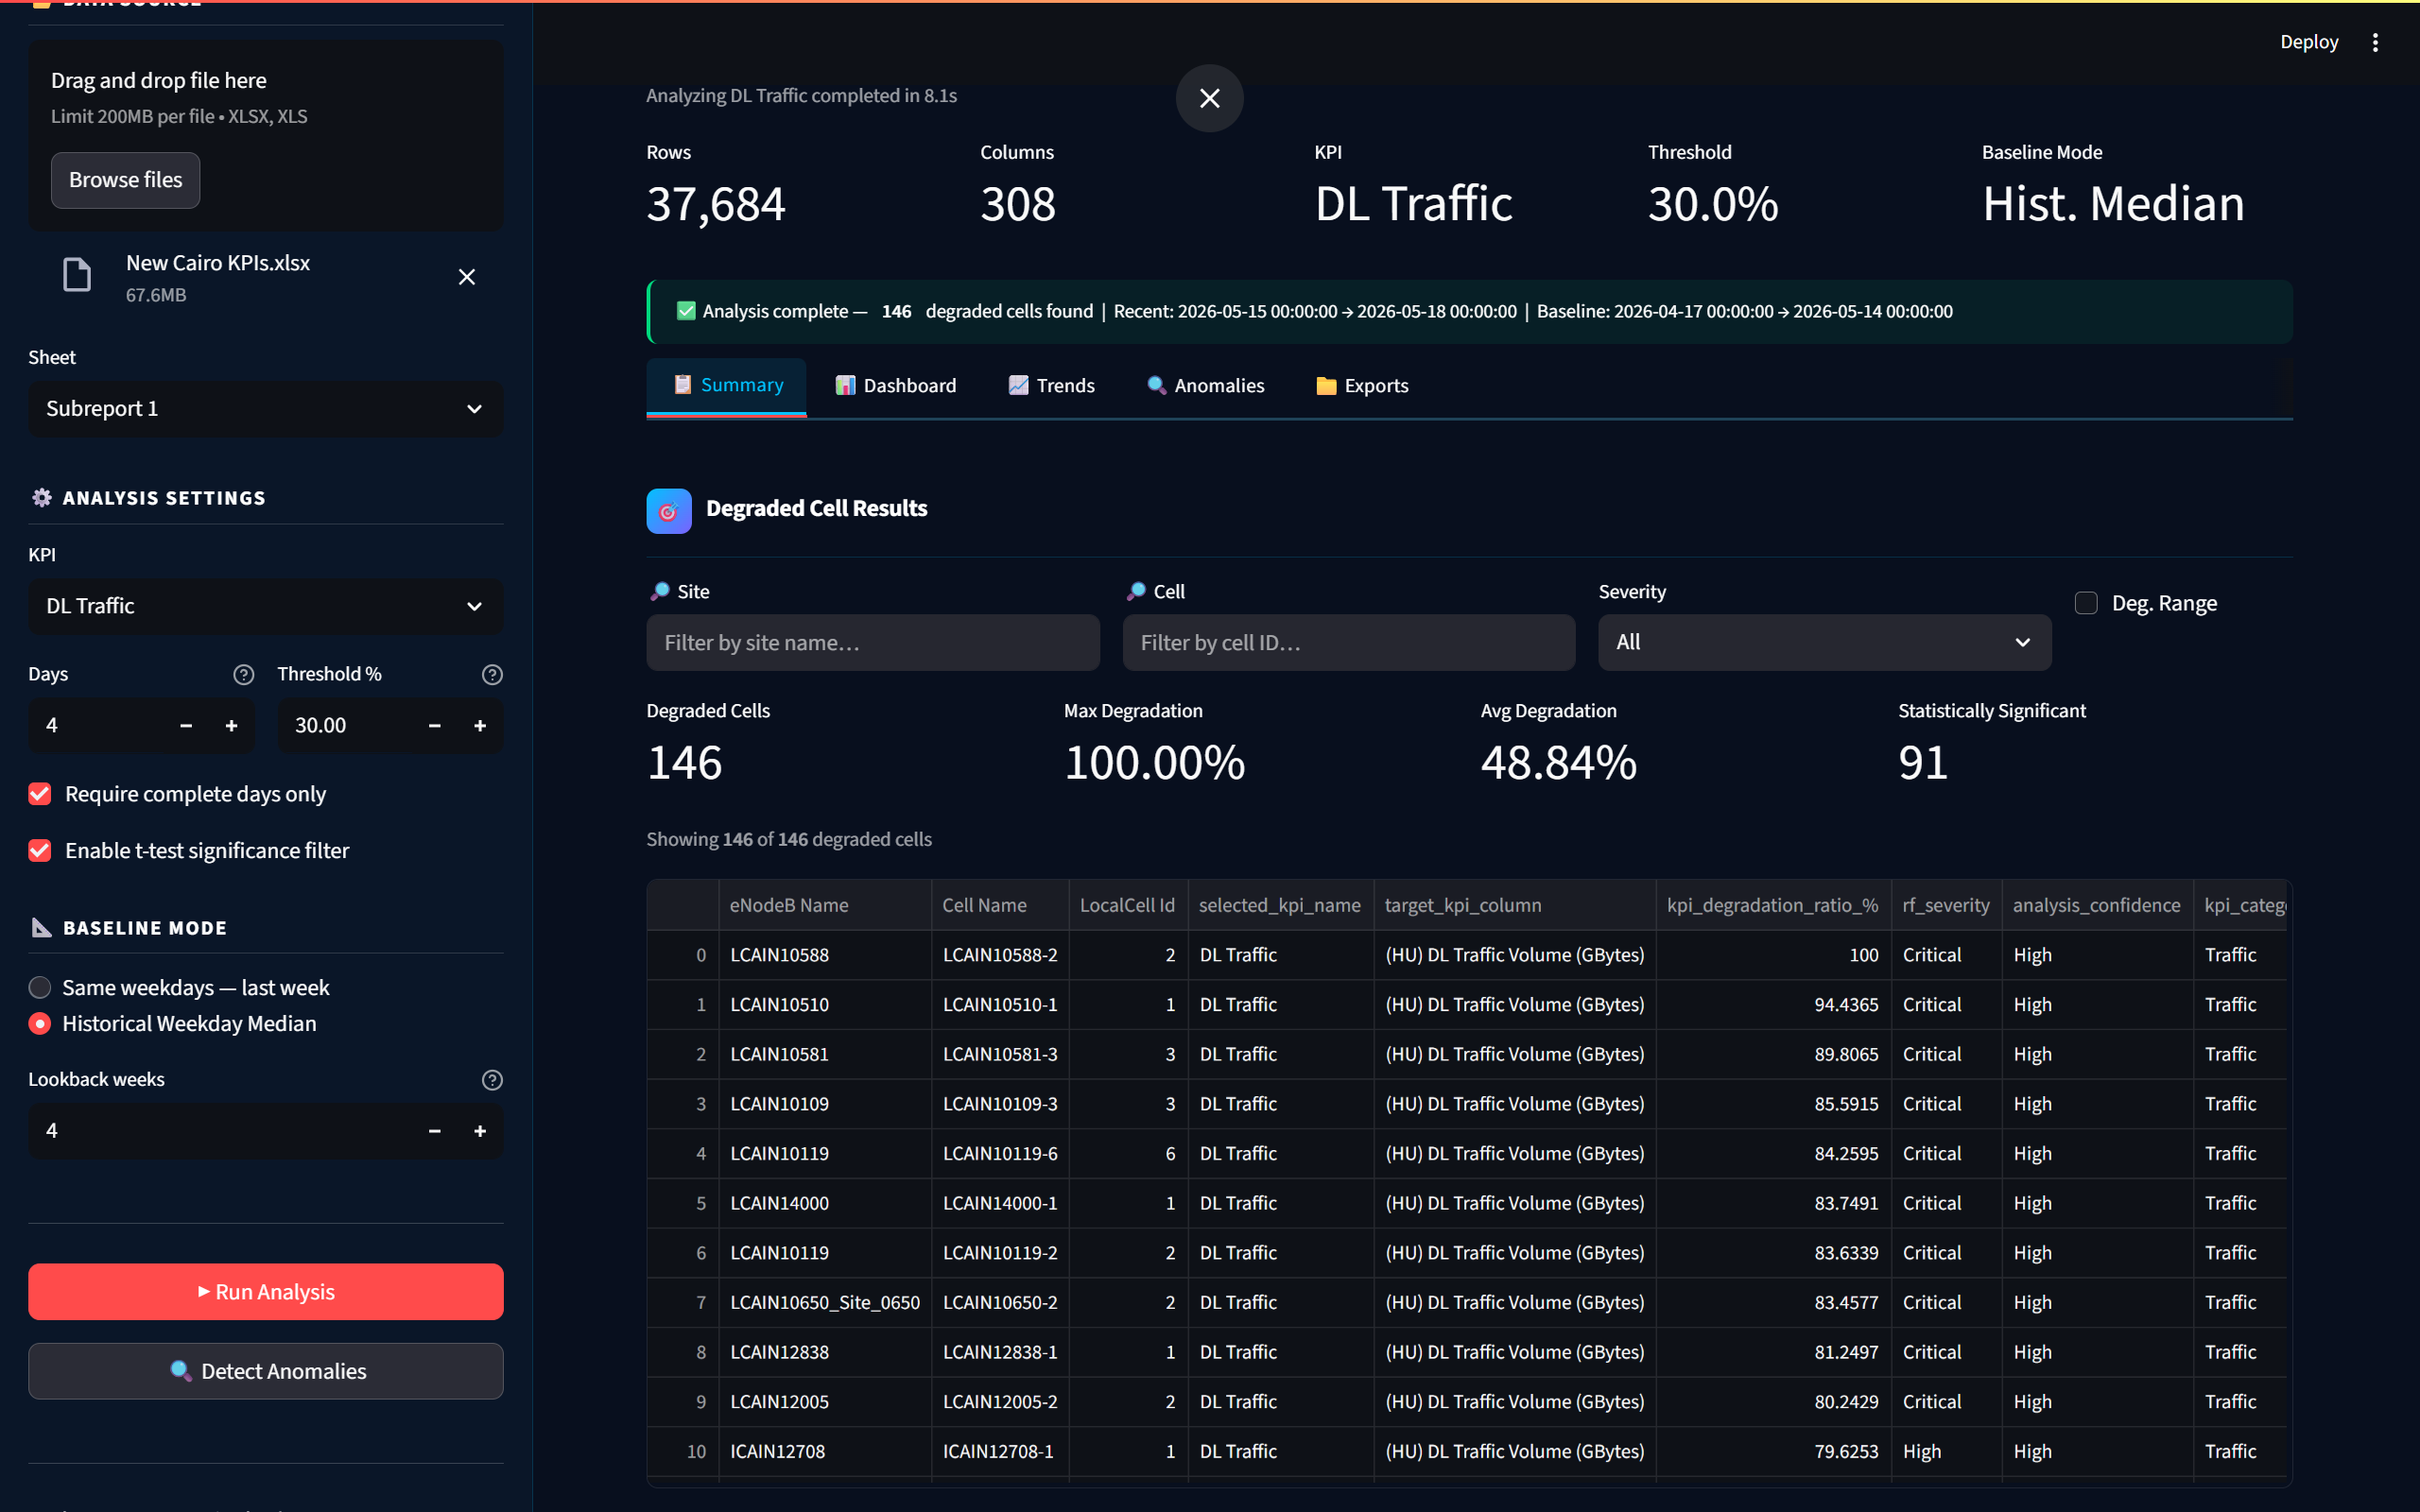
\includegraphics[width=\textwidth]{figures/chapter04/severity_and_confidence.png}
    \caption{Severity and confidence metric panels showing the distribution of rf\_severity classifications and analysis\_confidence levels across all degraded cells detected in the New Cairo dataset analysis.}
    \label{fig:severity_confidence}
\end{figure}

%%%%%%%%%%%%%%%%%%%%%%%%%%%%%%%%%%%%%%%%%%%%%%%%%%%%%%%%%%%%%%%%%%%%%%%%%%%%%%%%
\section{Trend Analysis}

The Trends tab enables engineers to visualise the historical KPI time series for individual degraded cells, comparing the recent observation window against the historical baseline period. This visualisation supports engineering judgement about the trajectory of the degradation and assists in distinguishing acute step changes from gradual long-term trends.

Figure~\ref{fig:trend_analysis} presents the trend analysis view for a representative degraded cell, showing the KPI time series with baseline and recent window highlighted.

\begin{figure}[H]
    \centering
    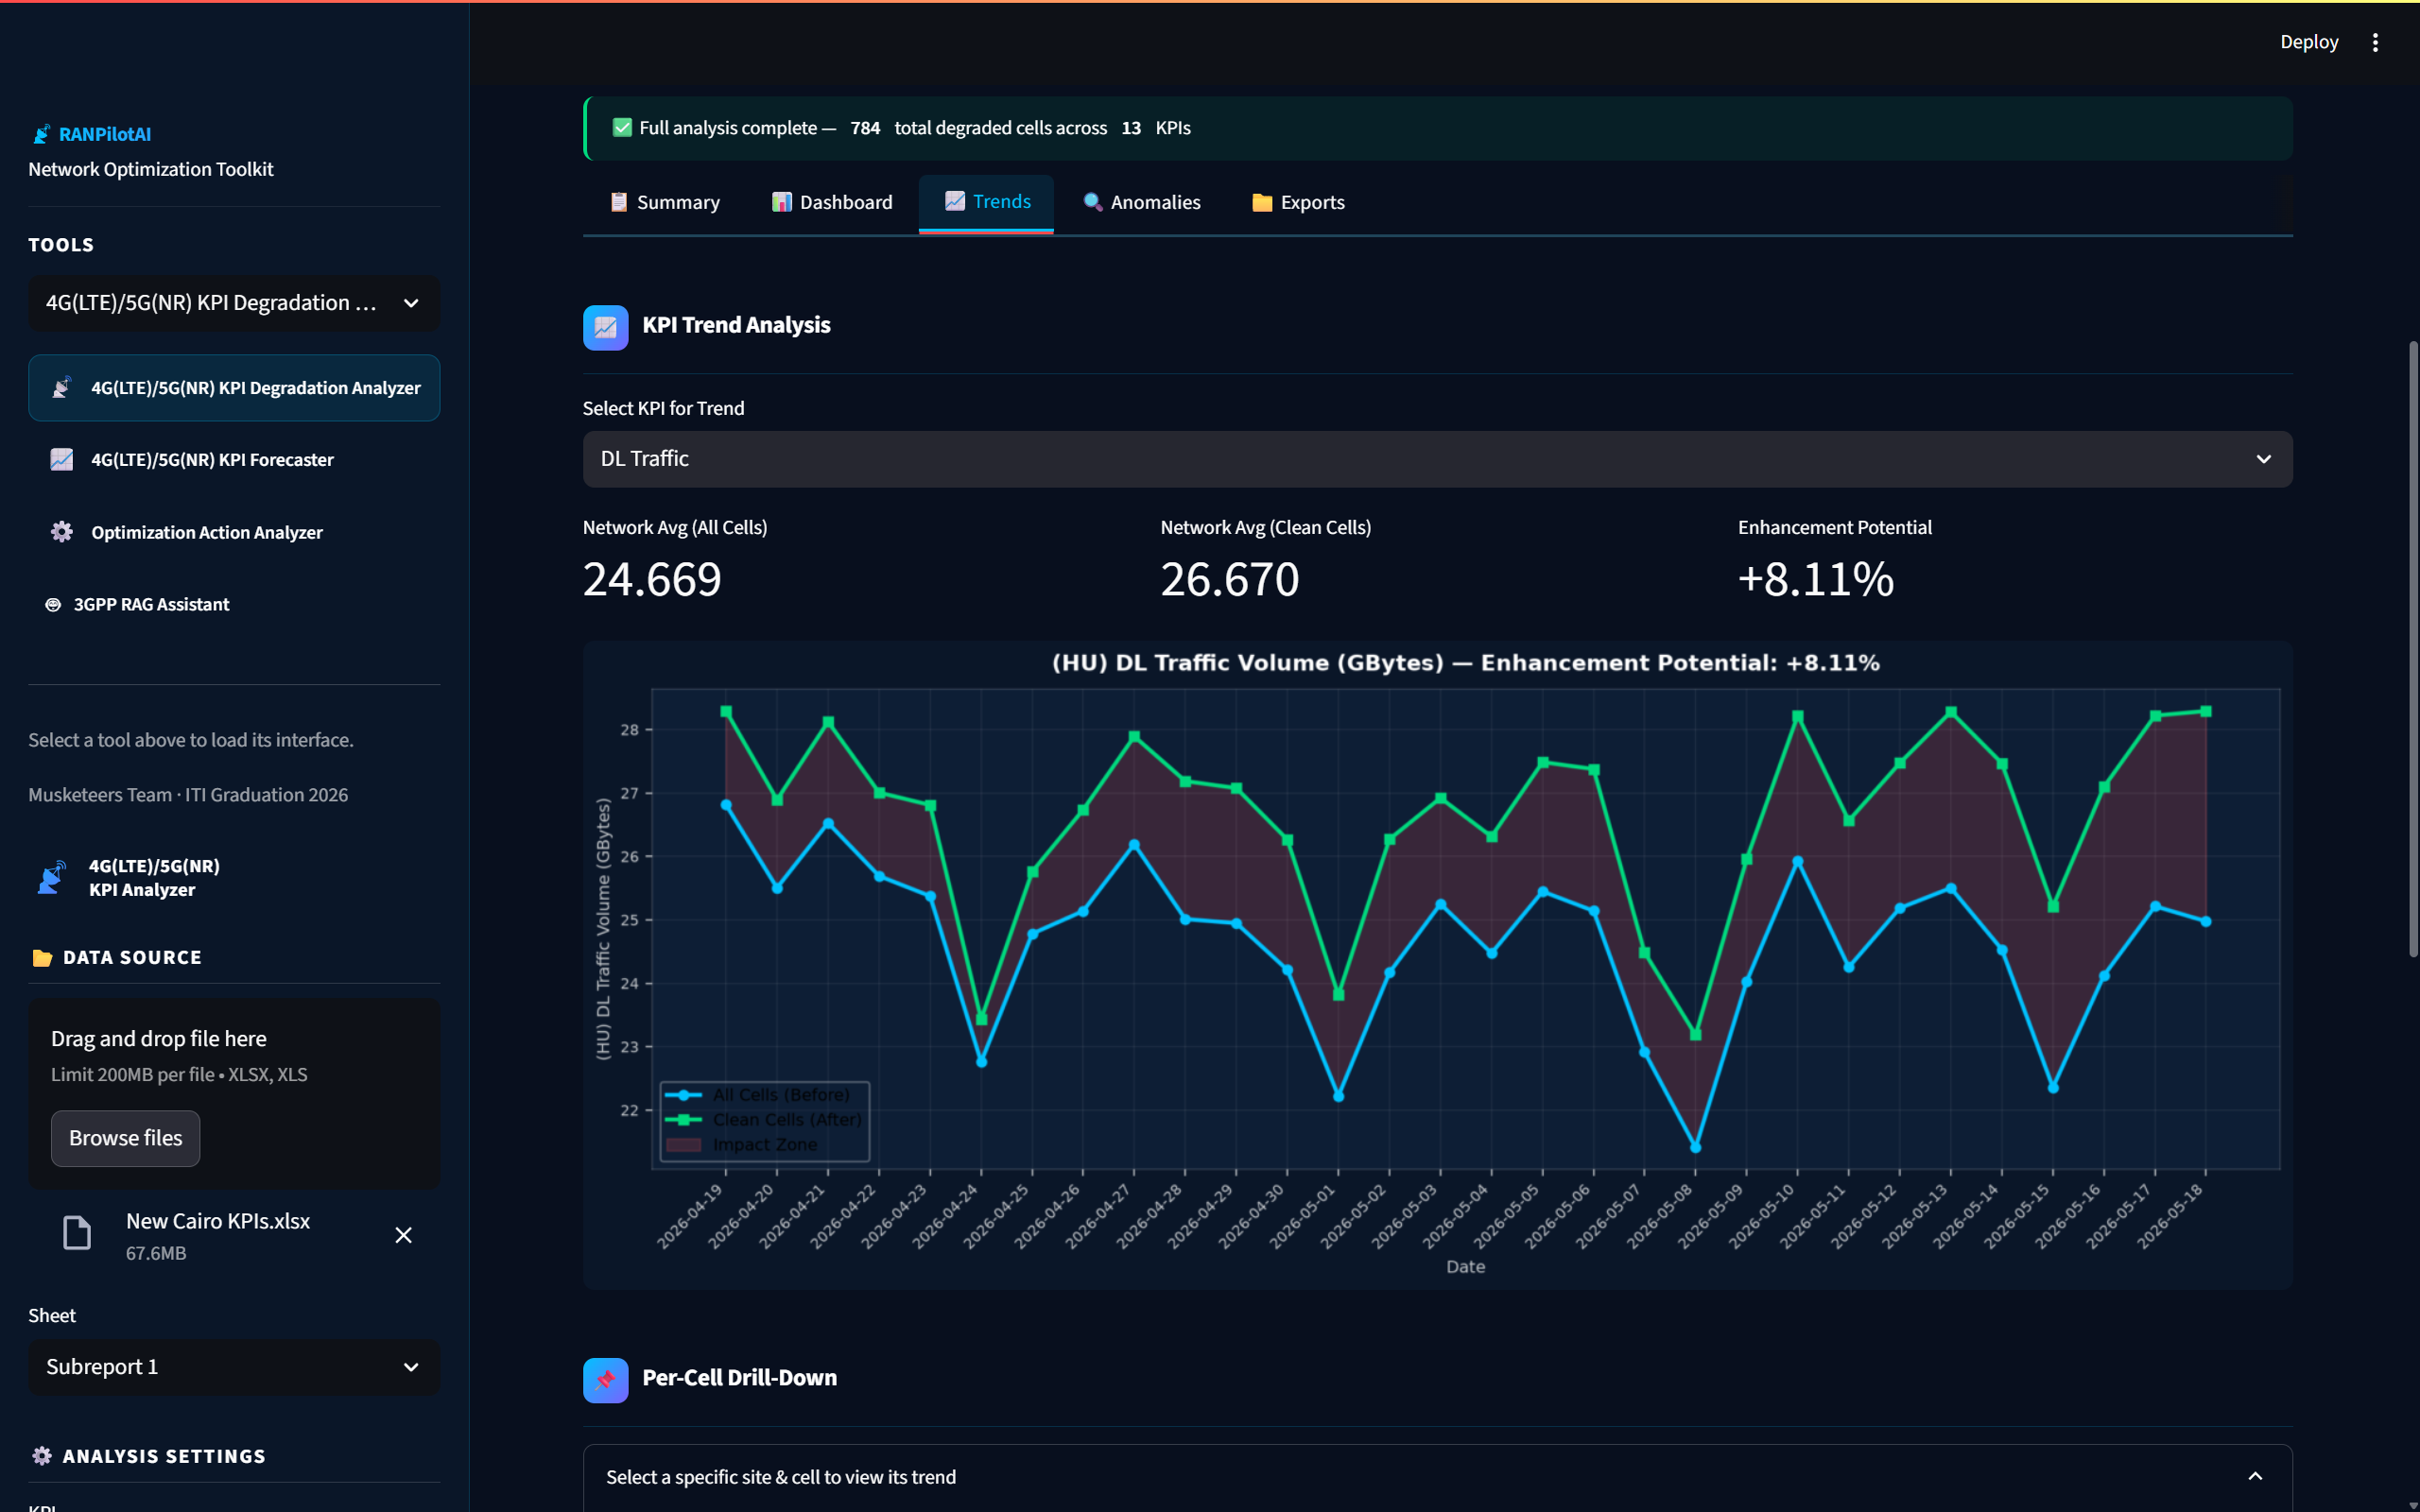
\includegraphics[width=\textwidth]{figures/chapter04/trend_analysis.png}
    \caption{Trend analysis view showing the KPI time series for a selected degraded cell, with the historical baseline period and recent observation window indicated. The before-and-after overlay enables visual assessment of degradation onset and trajectory.}
    \label{fig:trend_analysis}
\end{figure}

Figure~\ref{fig:trend_analysis_1} presents an additional trend analysis example illustrating the per-cell drill-down capability for a different KPI category.

\begin{figure}[H]
    \centering
    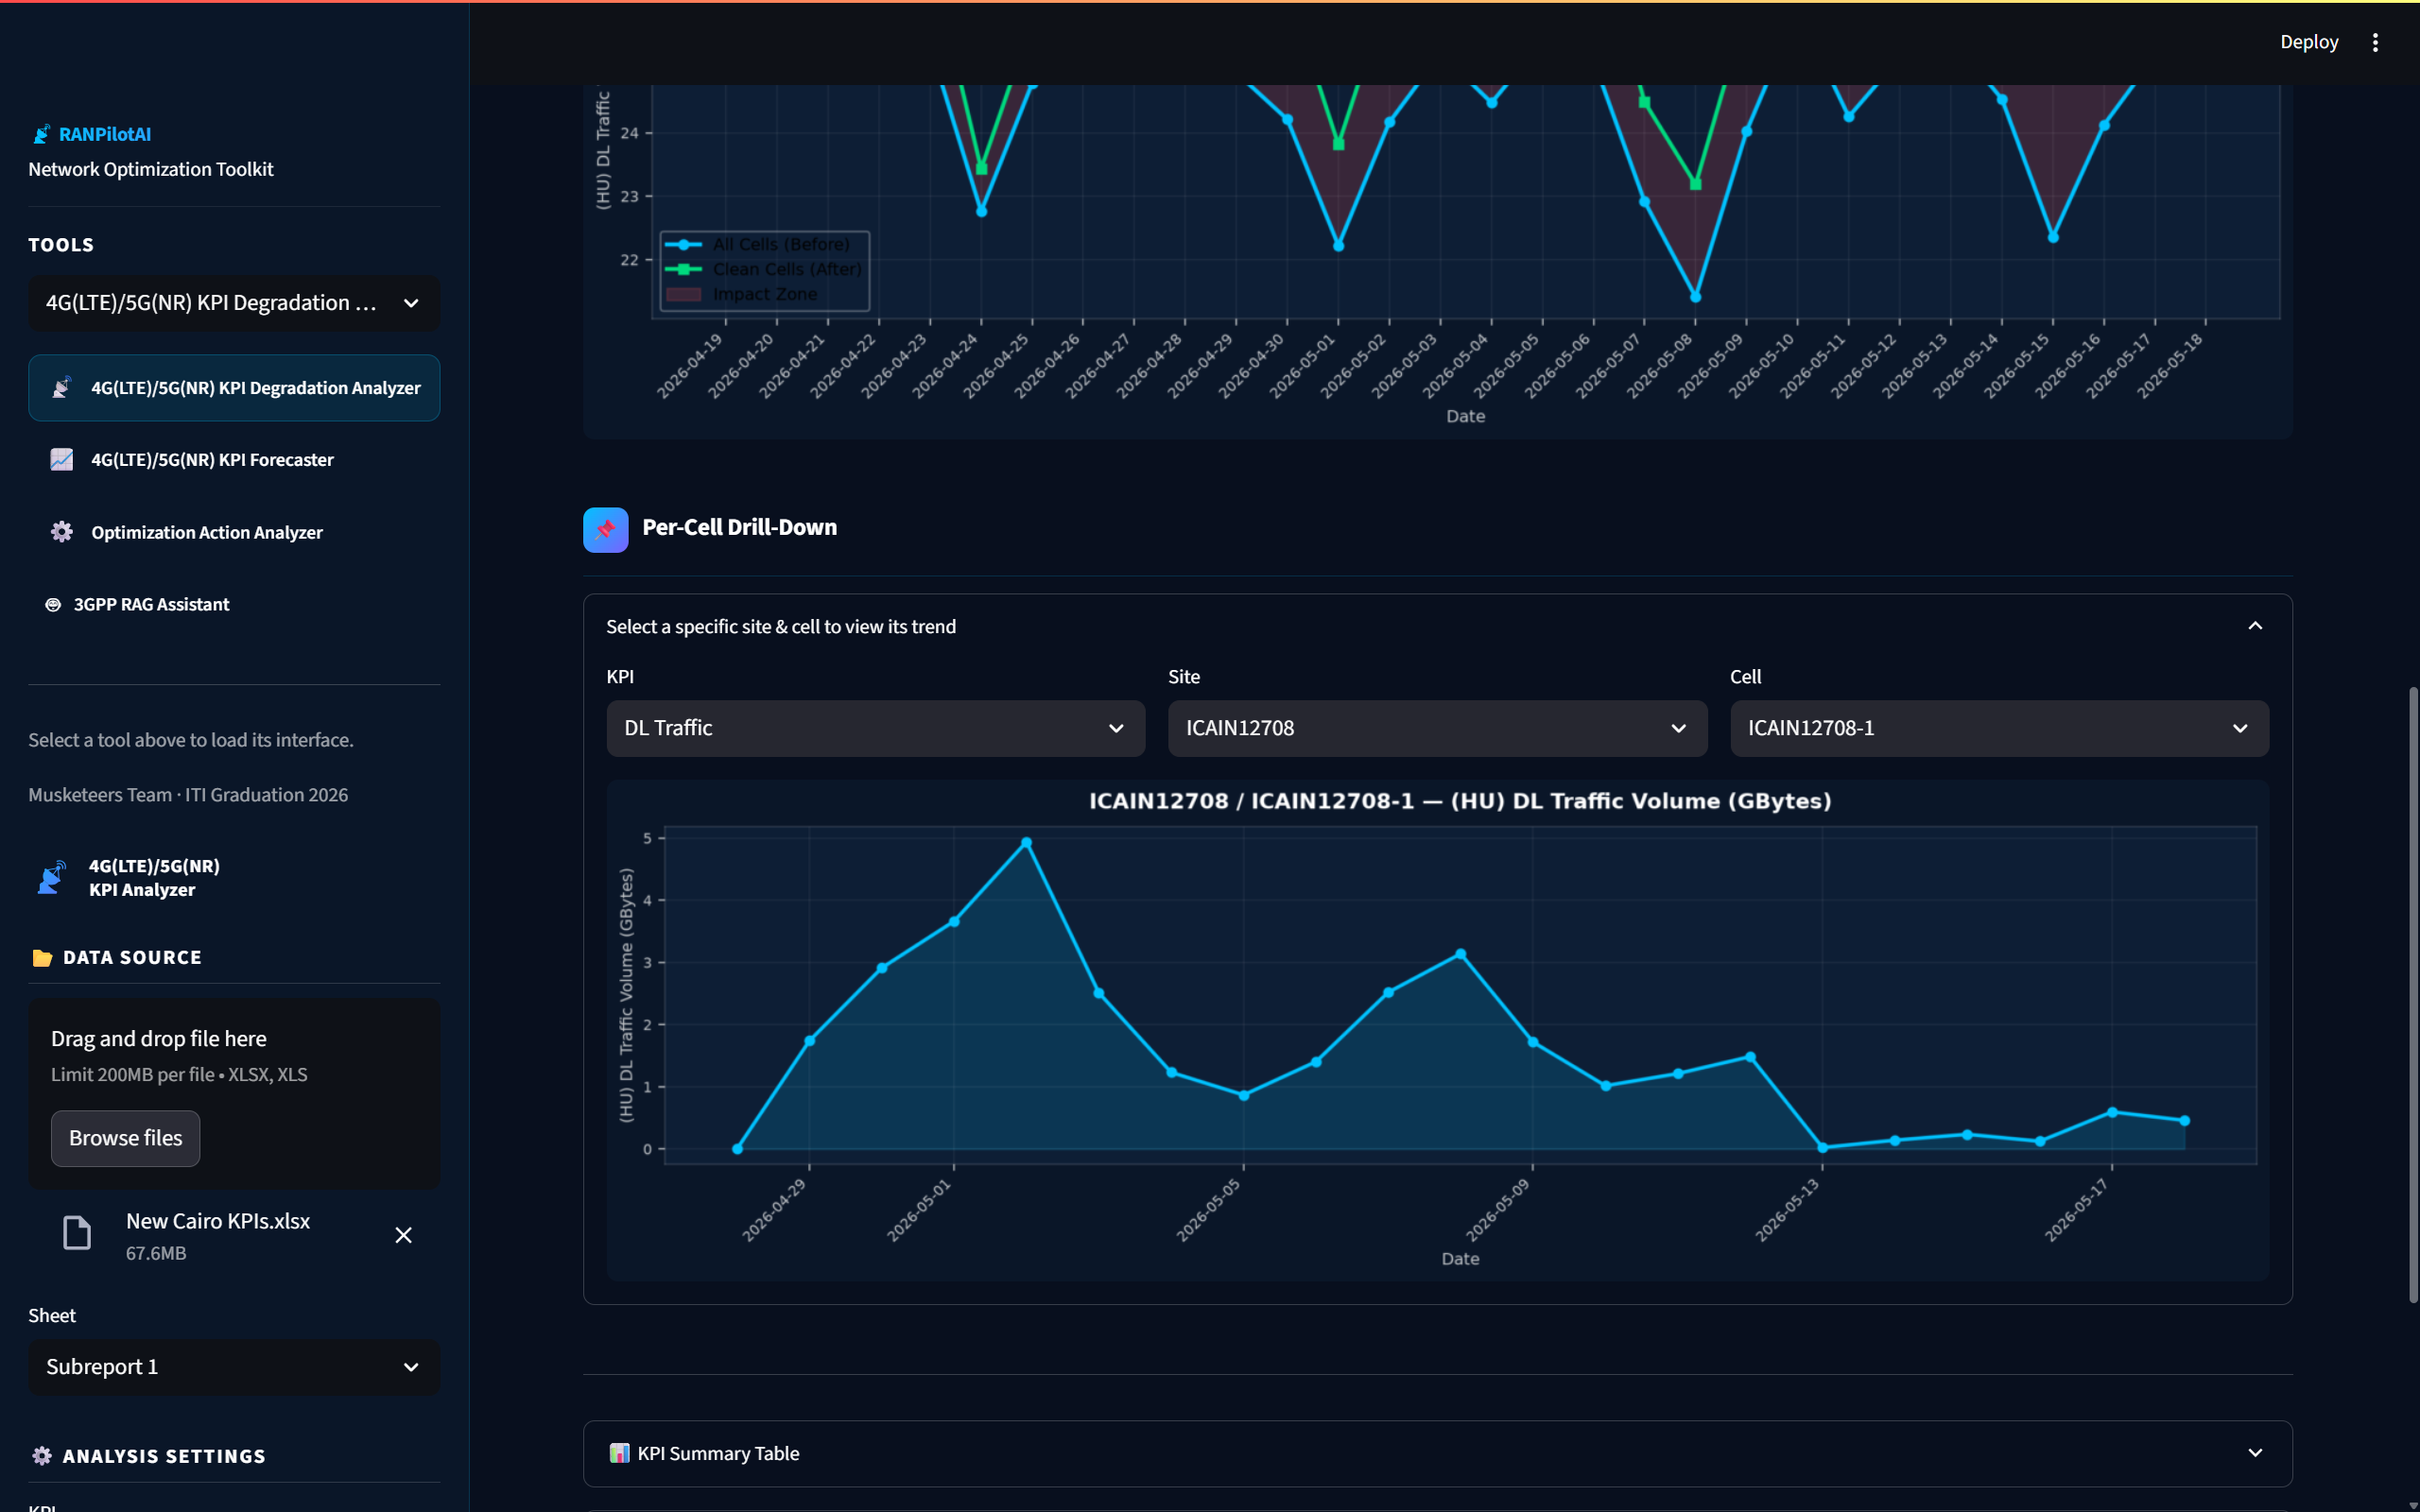
\includegraphics[width=\textwidth]{figures/chapter04/trend_analysis_1.png}
    \caption{Additional trend analysis drill-down showing multi-day KPI trajectory comparison between the baseline and recent periods for a second degraded cell, demonstrating the enhancement potential and before-after overlay visualisation capability.}
    \label{fig:trend_analysis_1}
\end{figure}

%%%%%%%%%%%%%%%%%%%%%%%%%%%%%%%%%%%%%%%%%%%%%%%%%%%%%%%%%%%%%%%%%%%%%%%%%%%%%%%%
\section{Anomaly Detection}

In addition to threshold-based degradation detection, the KPI Degradation Analyzer implements a statistical anomaly detection function that identifies zero-value and spike anomalies in the KPI time series using a 4-week rolling baseline. This function complements the main degradation detection pipeline by flagging transient anomalies that may not cross the threshold-based degradation criterion but nonetheless indicate operational issues requiring investigation.

Figure~\ref{fig:anomaly_detection} presents the anomaly detection output panel.

\begin{figure}[H]
    \centering
    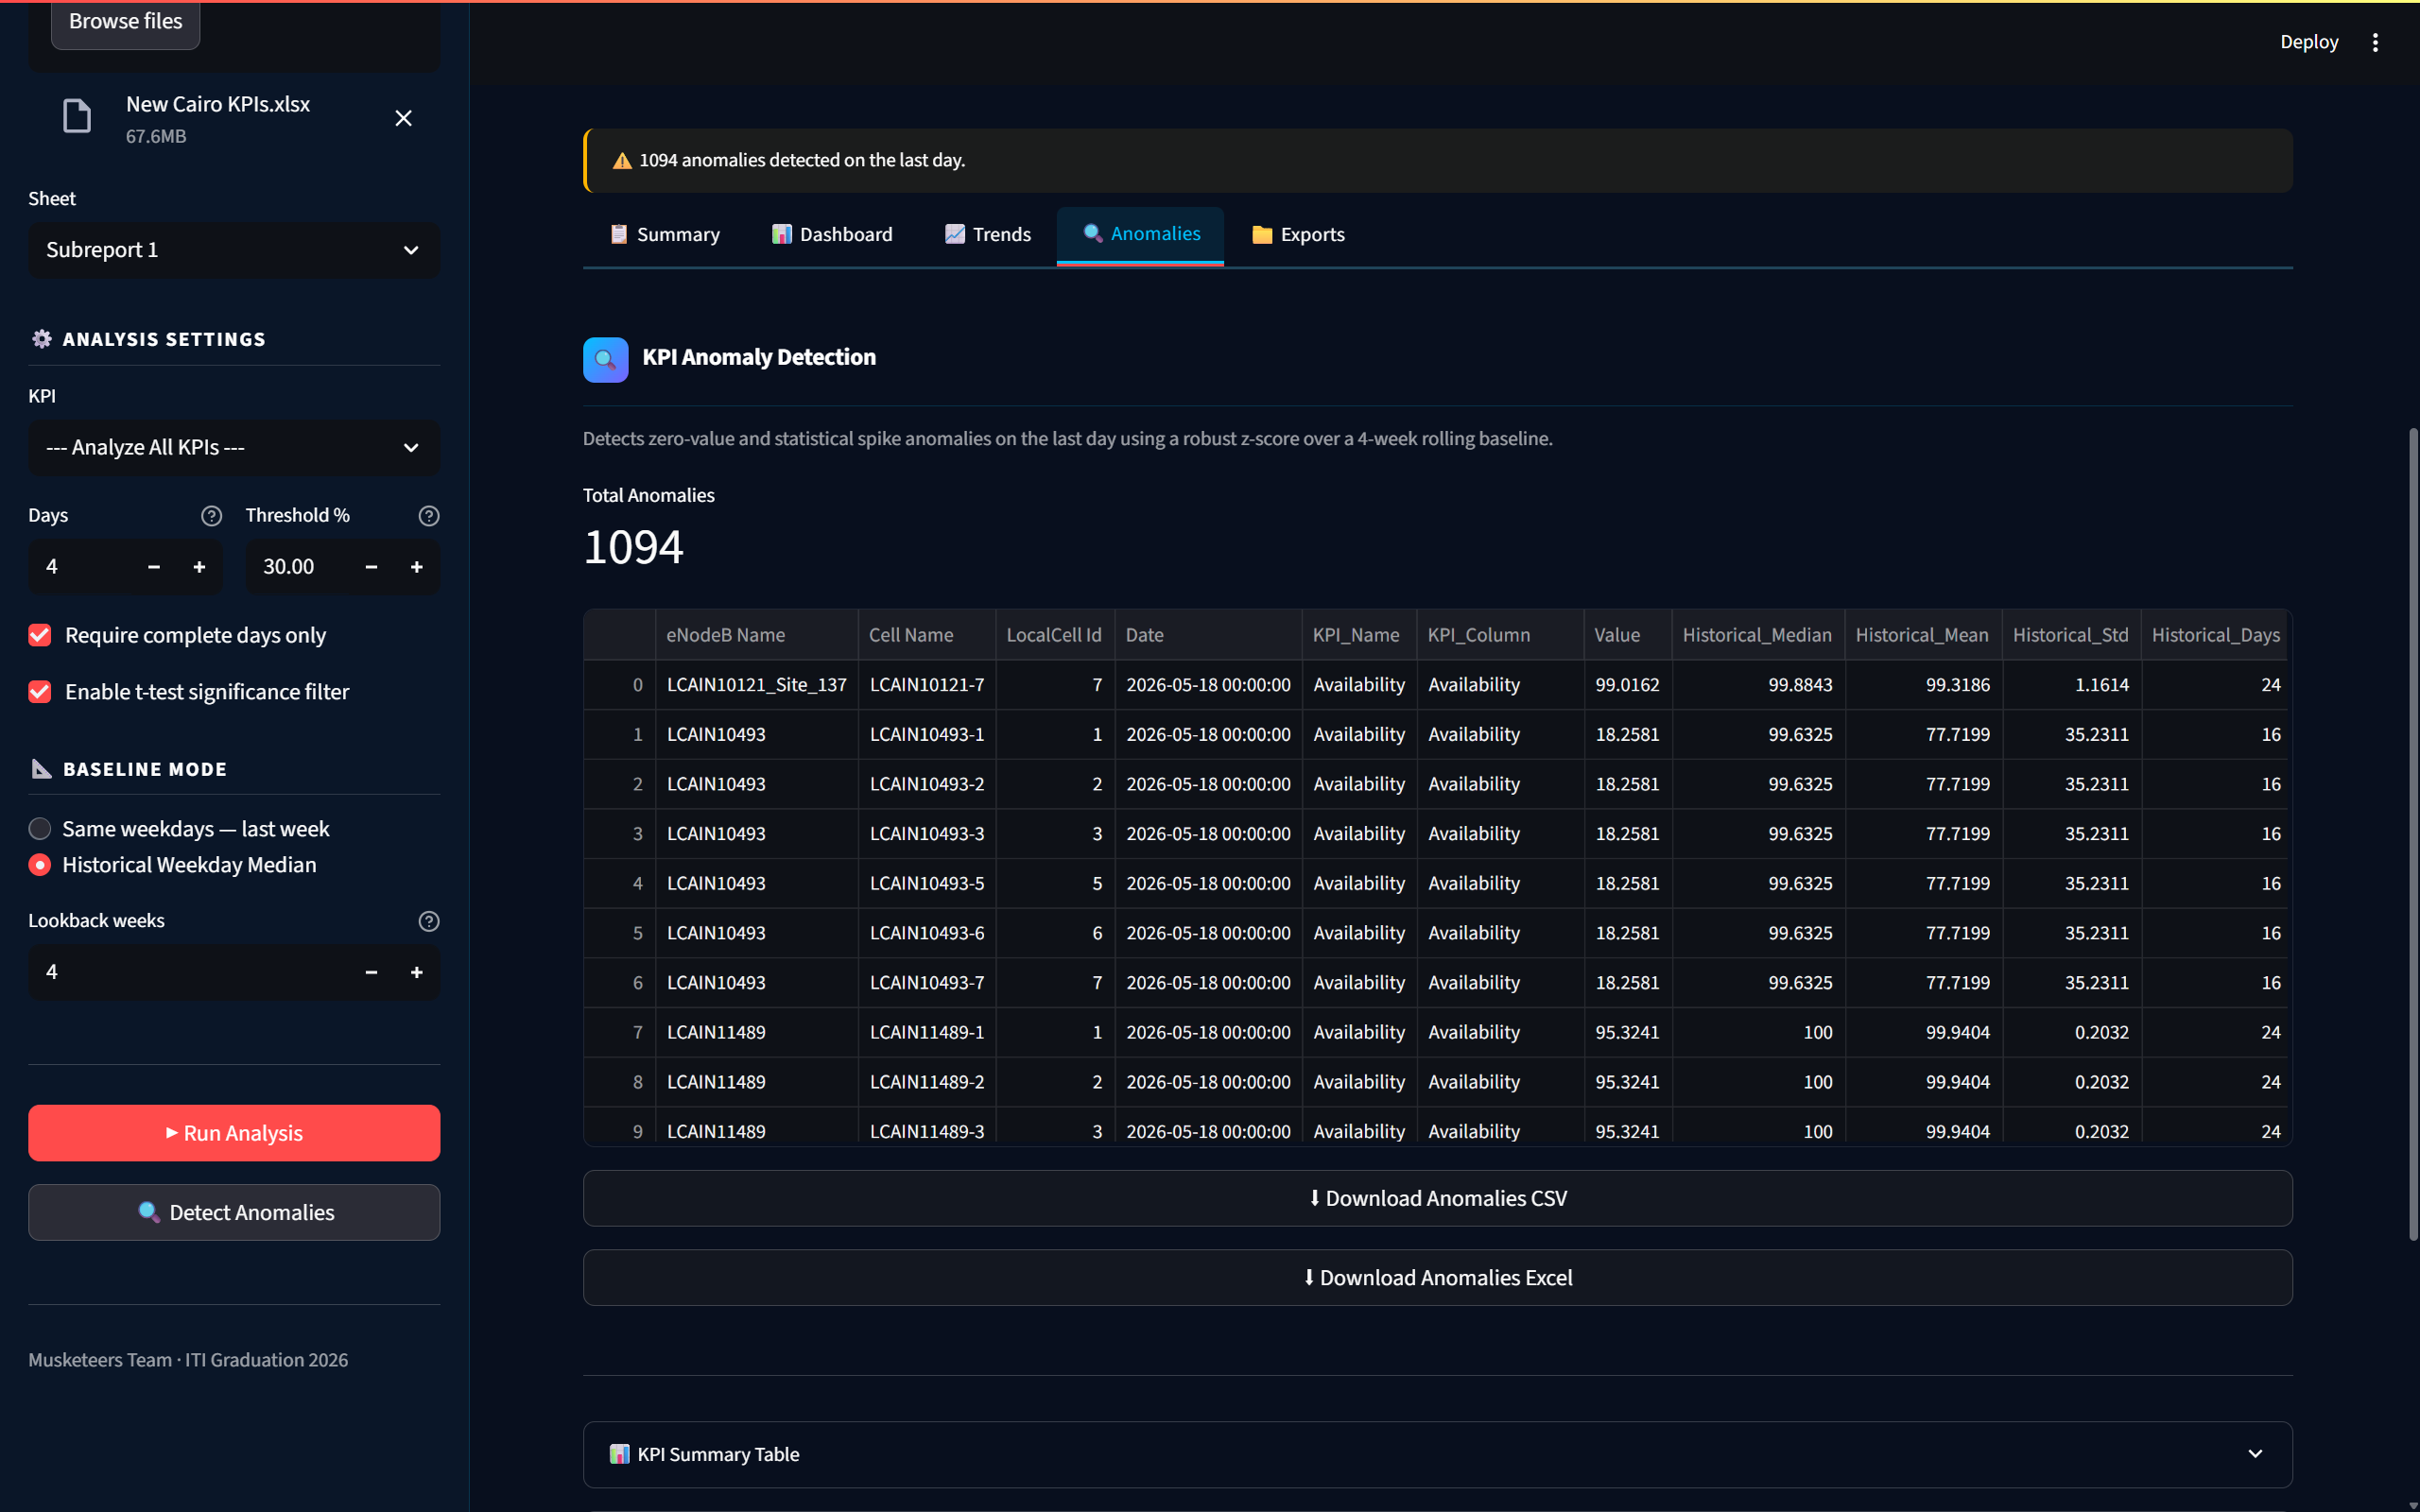
\includegraphics[width=\textwidth]{figures/chapter04/anomaly_detection.png}
    \caption{Anomaly detection panel showing zero-value and spike anomalies identified in the KPI time series across the analysed cell set, using a 4-week rolling baseline for comparison.}
    \label{fig:anomaly_detection}
\end{figure}

The anomaly detection engine applies the following classification criteria:

\begin{itemize}
    \item \textbf{Zero-value anomaly}: A counter reporting a value of zero on a day when the rolling mean is non-zero and no scheduled maintenance is recorded. Zero-value events for traffic or performance counters typically indicate a cell outage or data collection fault.
    \item \textbf{Positive spike anomaly}: A counter value exceeding a configurable number of standard deviations above the rolling mean, indicating an abnormal peak that may correspond to an interference event, a counter reset artefact, or a genuine traffic surge.
    \item \textbf{Negative spike anomaly}: A counter value falling a configurable number of standard deviations below the rolling mean, indicating an abrupt drop that may precede or accompany a sustained degradation.
\end{itemize}

%%%%%%%%%%%%%%%%%%%%%%%%%%%%%%%%%%%%%%%%%%%%%%%%%%%%%%%%%%%%%%%%%%%%%%%%%%%%%%%%
\section{Export Options}

The Exports tab provides multiple output format options enabling engineers to incorporate the analysis results into existing operational workflows and reporting templates. Figure~\ref{fig:export_options} presents the primary export panel.

\begin{figure}[H]
    \centering
    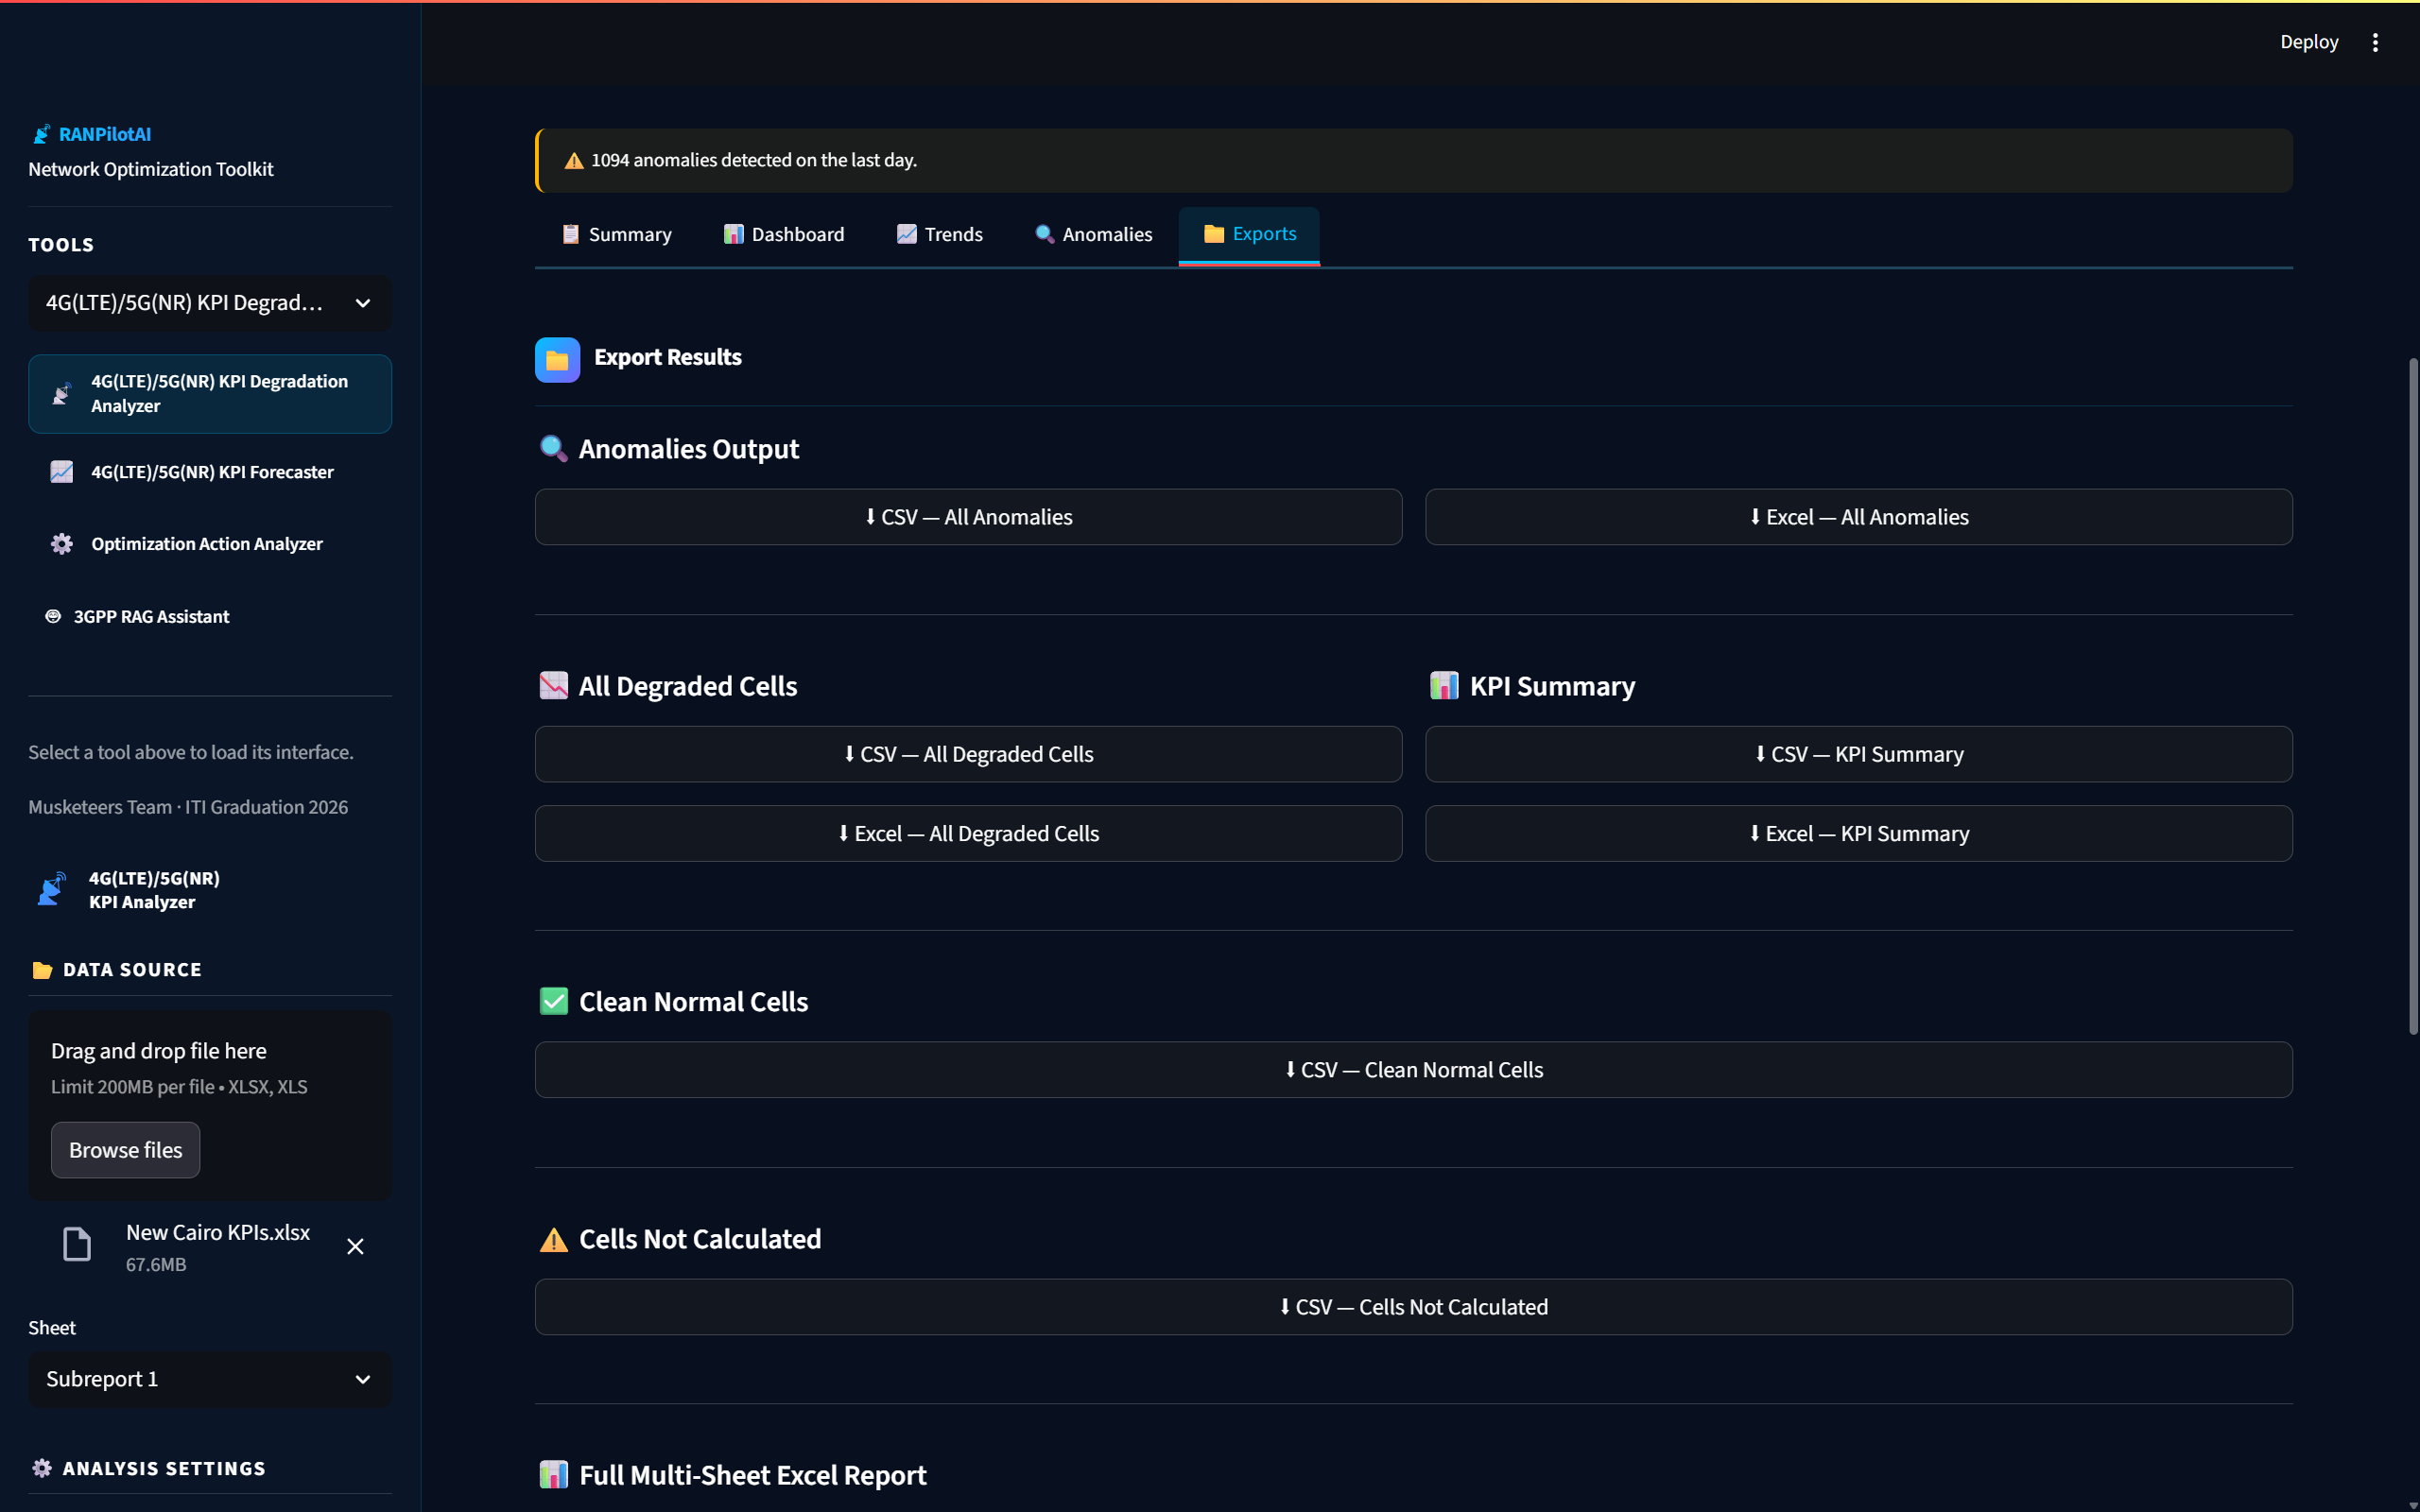
\includegraphics[width=\textwidth]{figures/chapter04/export_options.png}
    \caption{Primary export options panel of the KPI Degradation Analyzer, providing download buttons for Excel and Word format exports of the degradation analysis results.}
    \label{fig:export_options}
\end{figure}

Figure~\ref{fig:export_options_1} presents the additional export options including CSV format and chart export capabilities.

\begin{figure}[H]
    \centering
    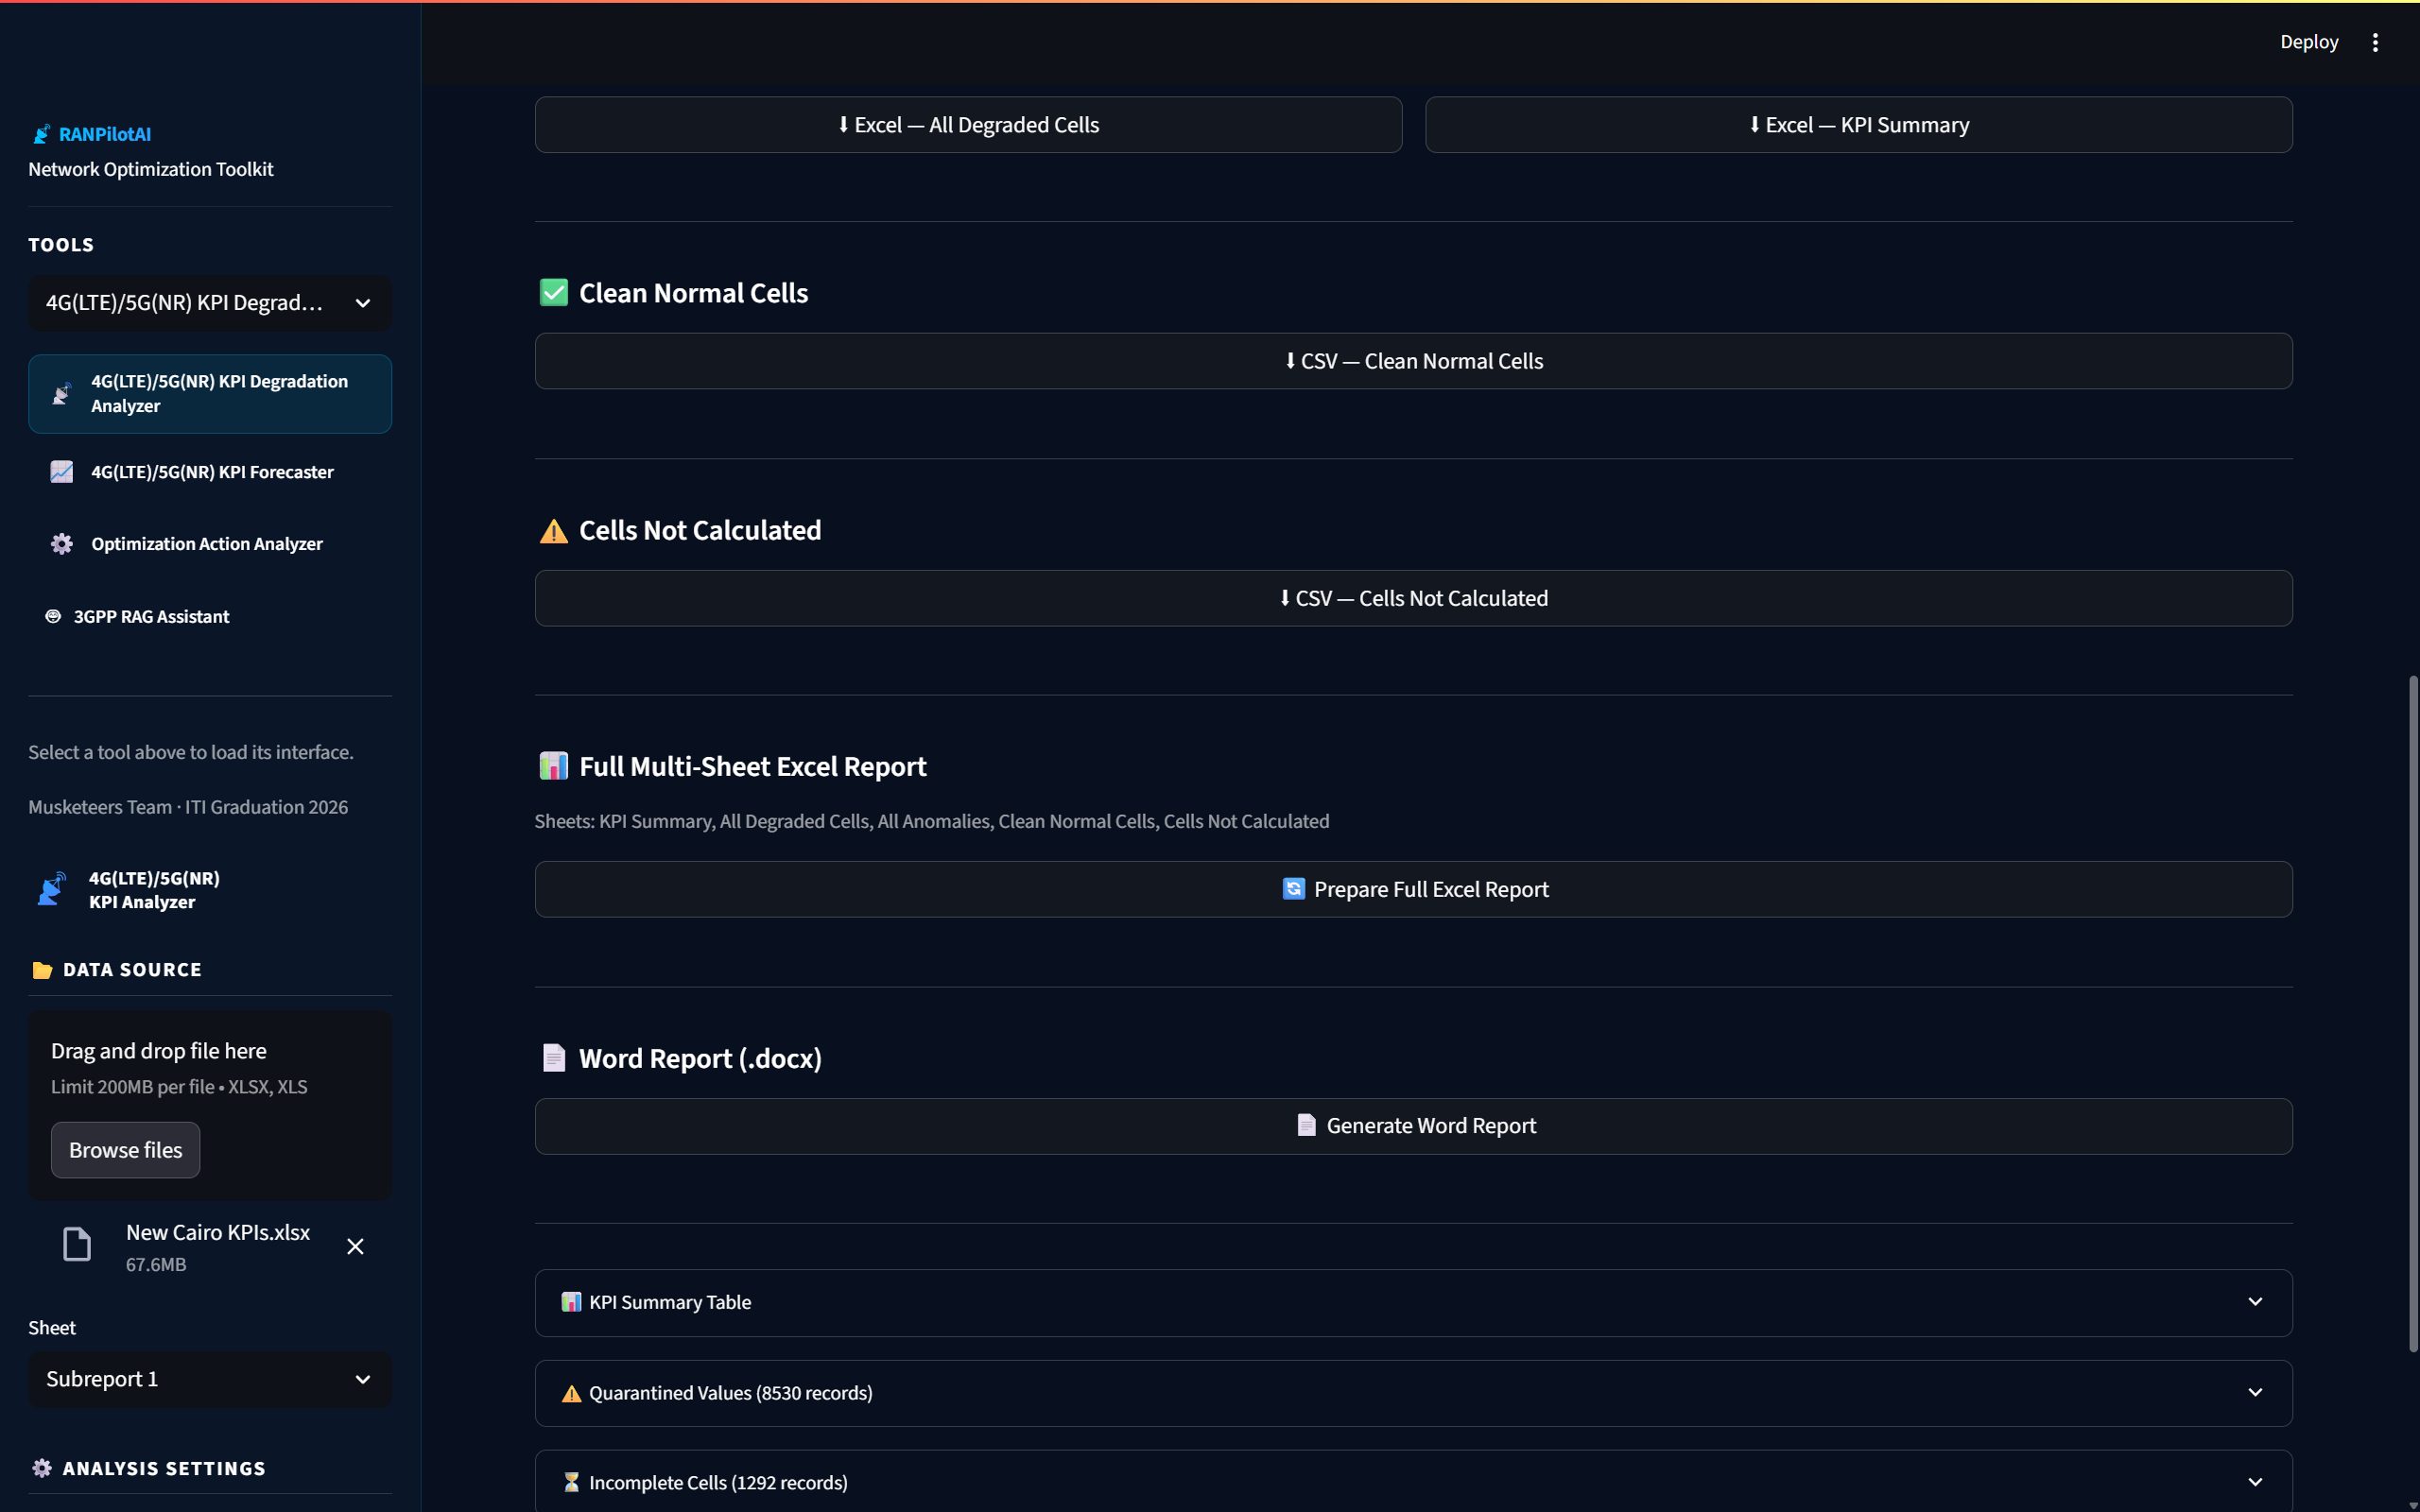
\includegraphics[width=\textwidth]{figures/chapter04/export_options_1.png}
    \caption{Additional export options providing CSV download and individual chart export capabilities for integration with external reporting and ticketing systems.}
    \label{fig:export_options_1}
\end{figure}

The following export formats are supported:

\begin{itemize}
    \item \textbf{Excel (XLSX)}: A formatted multi-sheet workbook containing the KPI summary table, the degraded cells detail table with all RCA output columns, and per-KPI result sheets. Cell values are conditionally formatted using red-green colour coding based on severity classification.

    \item \textbf{Word (DOCX)}: A formatted report document suitable for inclusion in network performance reports or incident analysis documentation. The Word export includes summary statistics, the KPI summary table, and the top degraded cells with root cause classifications.

    \item \textbf{CSV}: A flat comma-separated values file containing the complete degraded cells detail table, suitable for import into external analysis tools or network management systems.
\end{itemize}

%%%%%%%%%%%%%%%%%%%%%%%%%%%%%%%%%%%%%%%%%%%%%%%%%%%%%%%%%%%%%%%%%%%%%%%%%%%%%%%%
\section{Summary}

This chapter has presented the KPI Degradation Analyzer module of the RANPilotAI platform in detail. The module implements a three-layer analytical pipeline comprising a data quality engine, a statistical degradation detection engine, and an RF-aware root cause analysis engine. The pipeline processes raw KPI counter exports from LTE and 5G NR networks and produces structured degradation reports including severity classifications, confidence scores, root cause pattern identifications, and recommended next investigation steps.

The experimental validation of this module on the New Cairo LTE dataset, demonstrating the detection of 784 degraded cells across 13 KPI categories from a dataset of 37{,}684 rows and 308 columns, is presented in Chapter~9. The module successfully replaces a manual cell-by-cell analysis workflow with an automated, RF-aware analysis pipeline that runs to completion in seconds, producing consistent and interpretable output across all monitored KPI categories.
